\chapter{Рестарты зеркального спуска для относительно липшицевых задач с условием $\gamma$-роста}\label{ch:ch3}

\section{Введение}\label{sec:ch3/sect1}

    В предыдущих пунктах уже упоминались пессимистичные теоретические оценки скорости сходимости для негладких задач в пространствах больших размерностей. Распространенным подходом к этой проблеме служит выделение специальных классов задач, таких как условие острого минимума \cite{6, 1} и условие сильной выпуклости. 

    На основе проводимого сравнения указанных выше условий, в данной главе будут предложены рестарты для субградиентных методов, улучшающие полученные ранее оценки благодаря использованию аналога условия острого минимума.  Кроме того, предлагается некоторая релаксация для понятия острого минимума, включающая в себя условие квадратичного роста и использующая функцию Брэгмана для оценки удаленности от решения. 
    
    Пункт \ref{sec:ch3/sect3} обобщает использованные в предыдущей главе подходы для уточнения оценок скорости сходимости для сильно выпуклых задач и вводимое условие относительного $\gamma$-роста. В рамках данного пункта получены оценки скорости сходимости по значению и по аргументу функции, улучшающие рассмотренные ранее сублинейные оценки скорости сходимости, предложенные изначально в \cite{Bach_2012}. В последующем пункте \ref{sec:ch3/sect4} предложены улучшения для полученного метода, направленные на удобство его использования. В частности проведена заменена констант, использующих расстояние от начальной точки до точного решения, на их оценки. Также предложен критерий остановки на каждом из рестартов, который может значительно сократить общее количество итераций на практике.

 \section{Экспериментальное сравнение скорости сходимости для задачи поиска покрывающего шара наименьшего радиуса двух субградиентных методов при различных дополнительных условиях}  \label{sec:ch3/sec2}

    В данном пункте предложен анализ экспериментального сравнения двух субградиентных методов, использующих различные дополнительные условия:
    \begin{enumerate}
        \item сильной выпуклости,
        \item условия острого минимума.
    \end{enumerate}
    Преимущества и оценки в сильно выпуклой постановке рассматривались ранее в \ref{sec:ch2/sec4} и являются продолжением результатов в \cite{Bach_2012}.

    Приведем без доказательства результат, полученный моими коллегами, (см. теорему 1 из \cite{sharp22}) который полезен для дальнейшего анализа экспериментально полученных результатов. Напомним, что в работе рассматриваются задачи вида
    \begin{gather}\label{min_q}
        \min_{x\in Q} f(x),
    \end{gather}
    где $Q$ --- выпуклое замкнутое подмножество $\mathbb{R}^{n}$. 
    
    Для сравнения скорости сходимости метода \eqref{orig_2} и полученной в теореме \ref{ThmBachAdaptive} оценки с результатом, полученным моими соавторами, в теореме \ref{theorem1} для задач с $\Delta$-острым минимумом. Напомним определение острого минимума. Говорят, что $f$ удовлетворяет условию острого минимума, если
    \begin{gather}\label{sm}
        f(x) - f(x_*) \geq \alpha \min_{x_* \in X_*} \|x- x_*\|_2 \quad \forall x \in Q
    \end{gather}
    для некоторого фиксированного $\alpha >0$ и $f(x_*) = f^* = \min\limits_{x\in Q} f(x)$ для всякого $x_* \in X_*$, где $Q$ --- выпуклое и замкнутое подмножество $\mathbb{R}^n$, $X_*$ --- компакт и $\|\cdot\|_2$ --- евклидова норма. 
    
    При таком допущении моими соавторами в работе \cite{sharp22} в теореме \ref{theorem1} был предложен субградиентный метод с гарантией  линейной скорости сходимости в случае доступности информации о точном значении $f^*$ \cite{Polyak1969} без использования в теоретических оценках скорости сходимости  параметра размерности пространства. Условие острого минимума верно, например, для задачи проектирования точки на выпуклый компакт. Однако требование доступности $f^*$ довольно ограничительно. В этой связи рассматривалось некоторое обобщение условия острого минимума
    \begin{gather}\label{eq_gen_sharp}
        f(x) - \overline{f} \geq \alpha \min_{x_* \in X_*} \|x - x_* \|_2 - \Delta,
    \end{gather}
    где $\overline{f}$  --- это некоторое приближение минимального значения функции $f^*$, причём $\overline{f} \geq f^*$. 

    \begin{theorem}\label{theorem1}
        Пусть $f$ --- выпуклая функция, и для задачи \eqref{min_q} с условием \eqref{eq_gen_sharp} используется метод \eqref{orig_2} c шагом
        $h_k = \dfrac{f(x_k) - \overline{f}}{\| \nabla f(x_k) \|_2^2}$. Пусть также $\forall i \geq 0$ верно $\alpha^2 \leq 2 \| \nabla f(x_i) \|_2^2$. Тогда верно неравенство:
        \begin{gather}\label{adaptive_estimate}
            \begin{aligned}
            \min_{x_* \in X_*} \|x_{k+1} - x_* \|_2^2 \leq &  \prod_{i=0}^k \left ( 1 - \frac{\alpha^2}{2 \| \nabla f(x_i) \|_2^2} \right ) \min_{x_* \in X_*} \|x_0 - x_* \|_2^2 + \\& 
            \qquad \qquad + \sum_{i=0}^{k-1} \prod_{j=i+1}^k \left ( 1 - \frac{\alpha^2}{2 \| \nabla f(x_j) \|_2^2} \right )\Delta_i + \Delta_k,
            \end{aligned}
        \end{gather}
        где $\Delta_k = \frac{\Delta^2}{2 \| \nabla f(x_k) \|_2^2}$ для всякого $k \geqslant 0$.
    \end{theorem}


    В данной постановке были проведены численные эксперименты. Поскольку для вышеупомянутых методов требуются различные свойства, то представлены 2 постановки для одной и той же, с геометрической точки зрения, задачи. Задача о наименьшем покрытии точек шаром для $2$-сильно выпуклой функции (уже использовалась ранее \eqref{sphere_cover_strongly})
    \begin{gather}
        f(x) := \max_{x\in Q}\left\{\|x - a_0\|_2^2, \|x - a_1\|_2^2, ..., \|x - a_m\|_2^2\right\},
    \end{gather}
    а также для не сильно выпуклой (но выпуклой) функции
    \begin{gather}\label{sphere_cover}
        f(x) := \max_{x\in Q}\left\{\|x - a_0\|_2, \|x - a_1\|_2, ..., \|x - a_m\|_2\right\}.
    \end{gather}

    Начнём с иллюстрации преимуществ адаптивной оценки метода \eqref{adaptive_estimation_f} из теоремы \ref{ThmBachAdaptive}. Будем рассматривать множество Q, которое равно евклидову шару с центром в 0. Начальная точка выбиралась случайно, но внутри Q. На рис. \ref{res_ex_strong_r5} ниже показано поведение и характер убывания для оригинальной оценки (\ref{orig_estimation_f}) --- сплошная линия, адаптивной оценки (\ref{adaptive_estimation_f}) --- штрих-пунктирная линия и непосредственно невязки по функции и по аргументу соответственно --- штриховая линия. На рис. \ref{res_ex_strong_r5} показано поведение глобальной оценки, адаптивной и невязки по функции и аргументу в случае ограниченного $Q \;(R = 5)$. Данный график наглядно демонстрирует, насколько более точной может оказаться адаптивная оценка (\ref{adaptive_estimation_f}) для задачи \eqref{sphere_cover_strongly}. Также показано поведение уже известных оценок (рис. \ref{r_20_q_6}) с учетом логарифмической шкалы для количества итераций.

    \begin{figure}[h]
        \minipage{0.49\textwidth}
        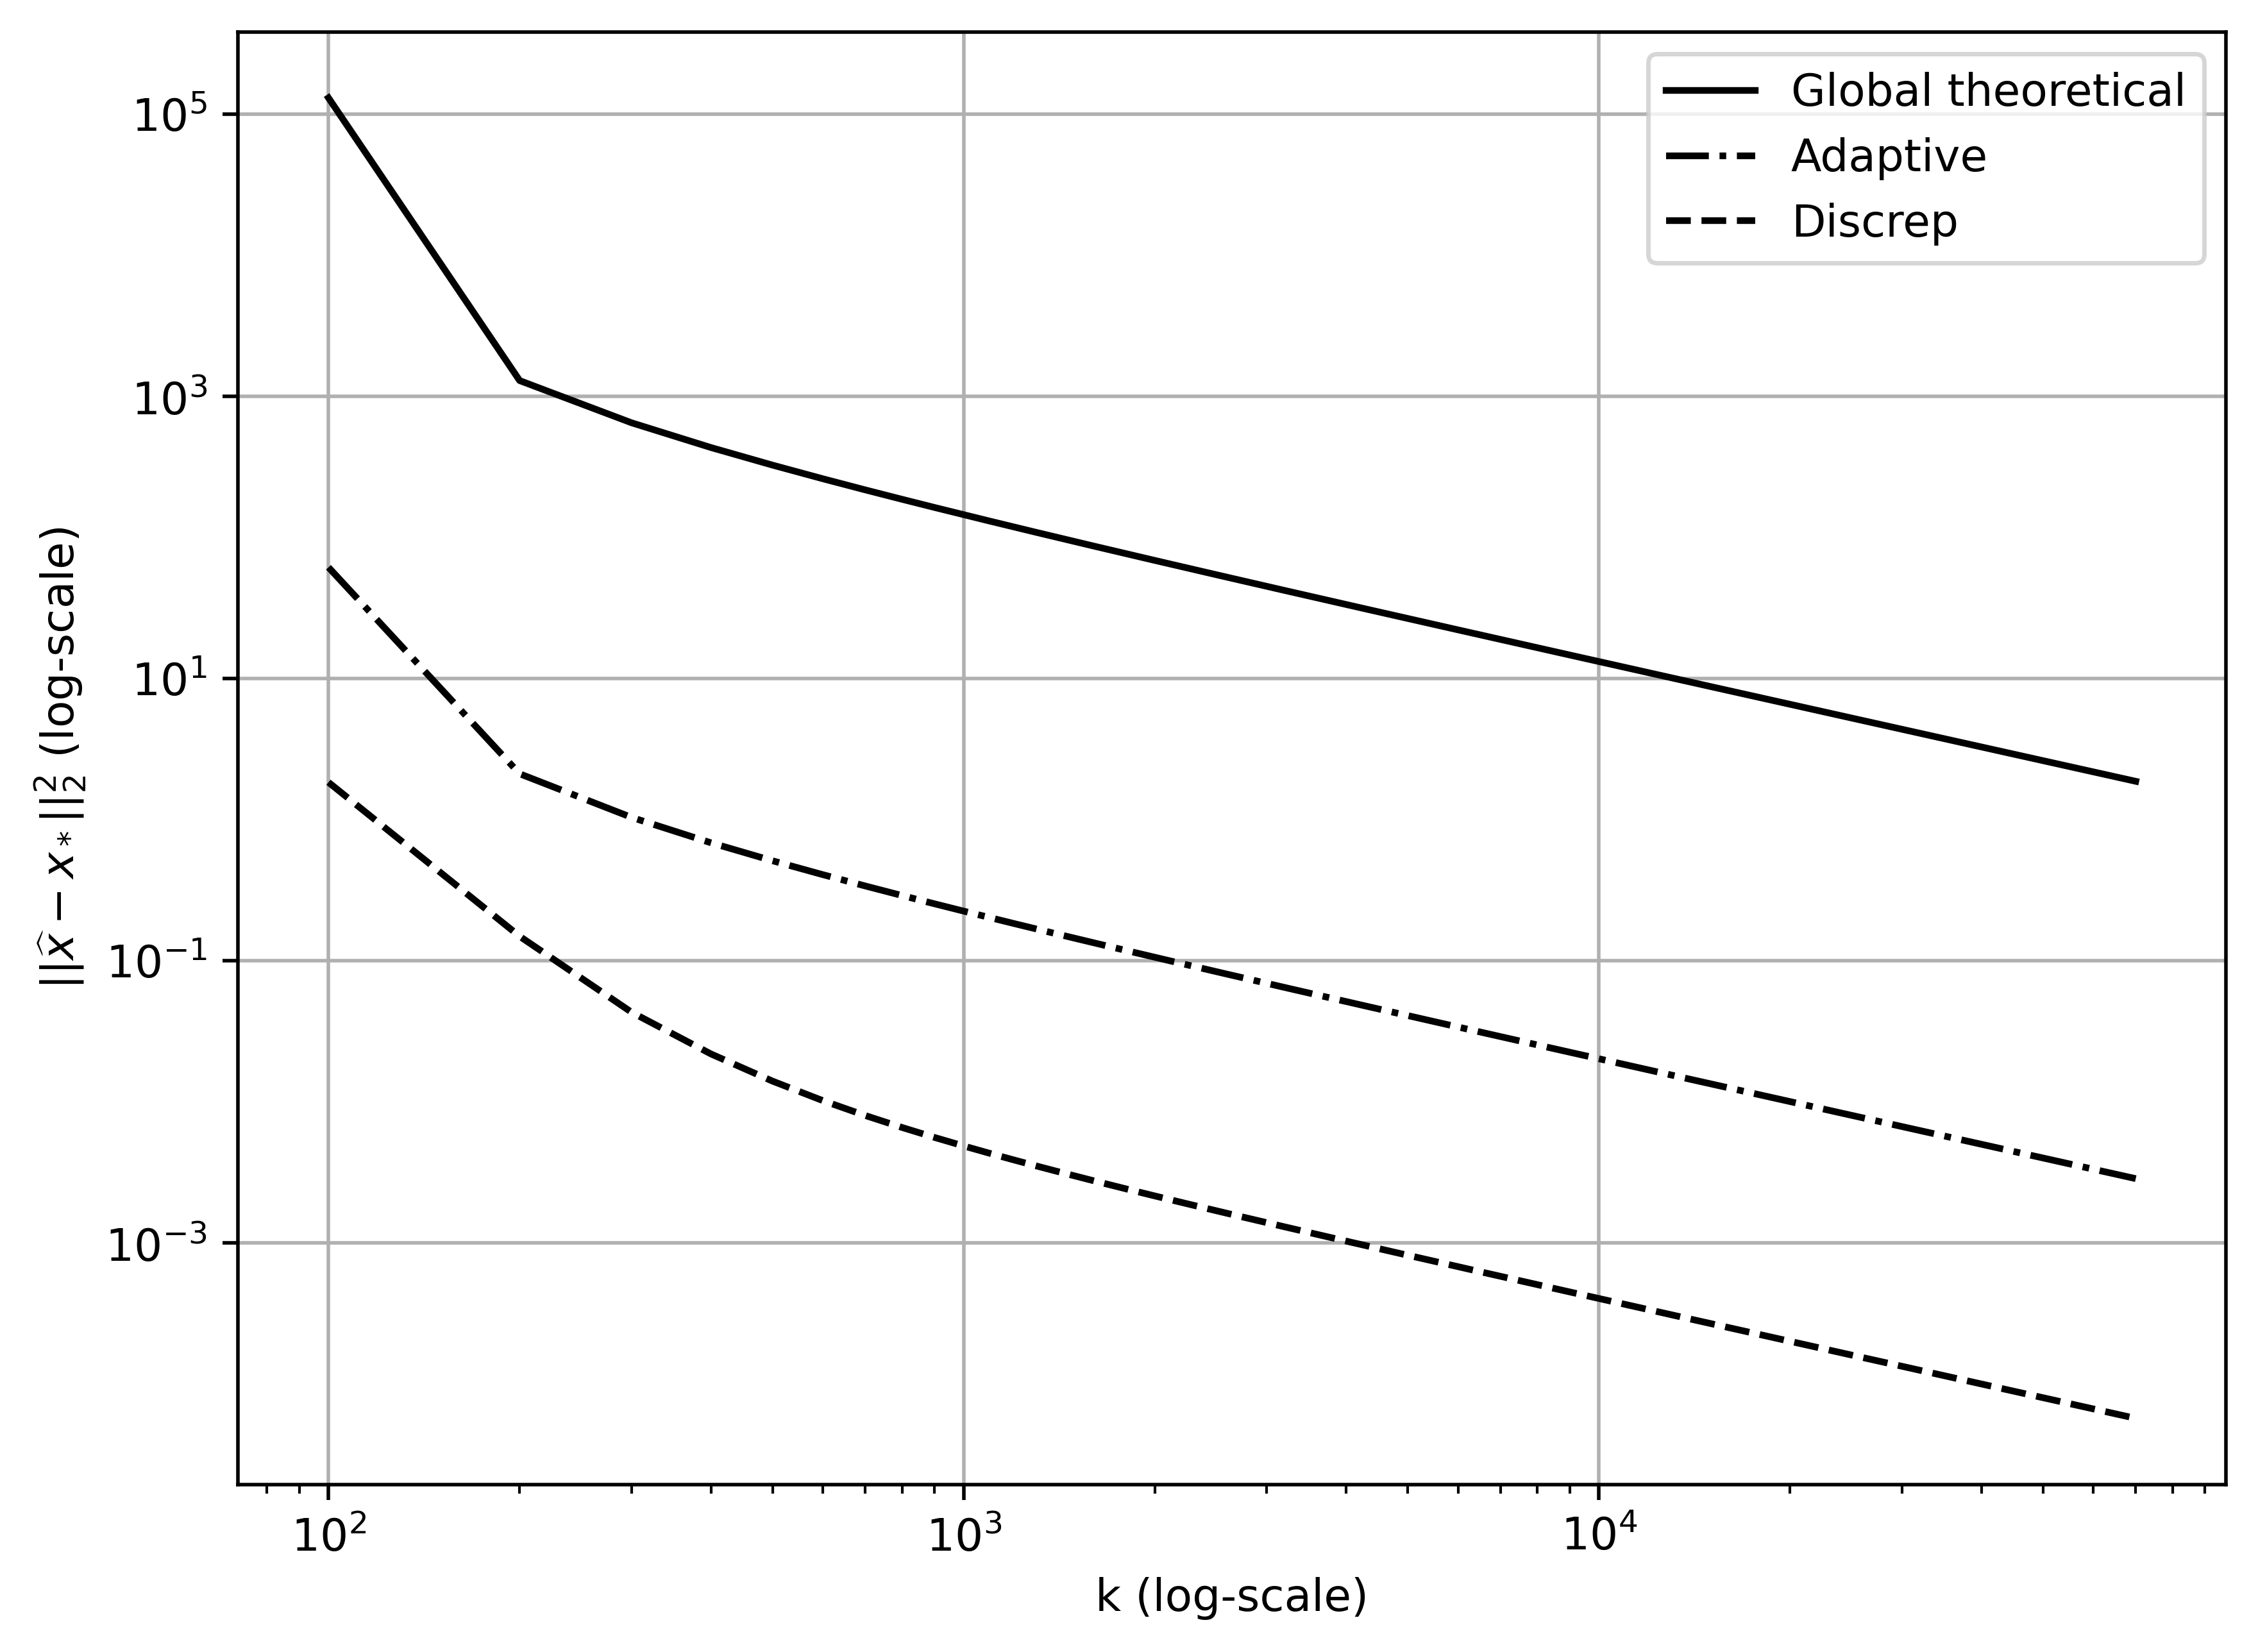
\includegraphics[width=\linewidth]{x_discr_rad_5_q_4_it_70_000_dim_1000.png}
        \endminipage\hfill
        \minipage{0.49\textwidth}
        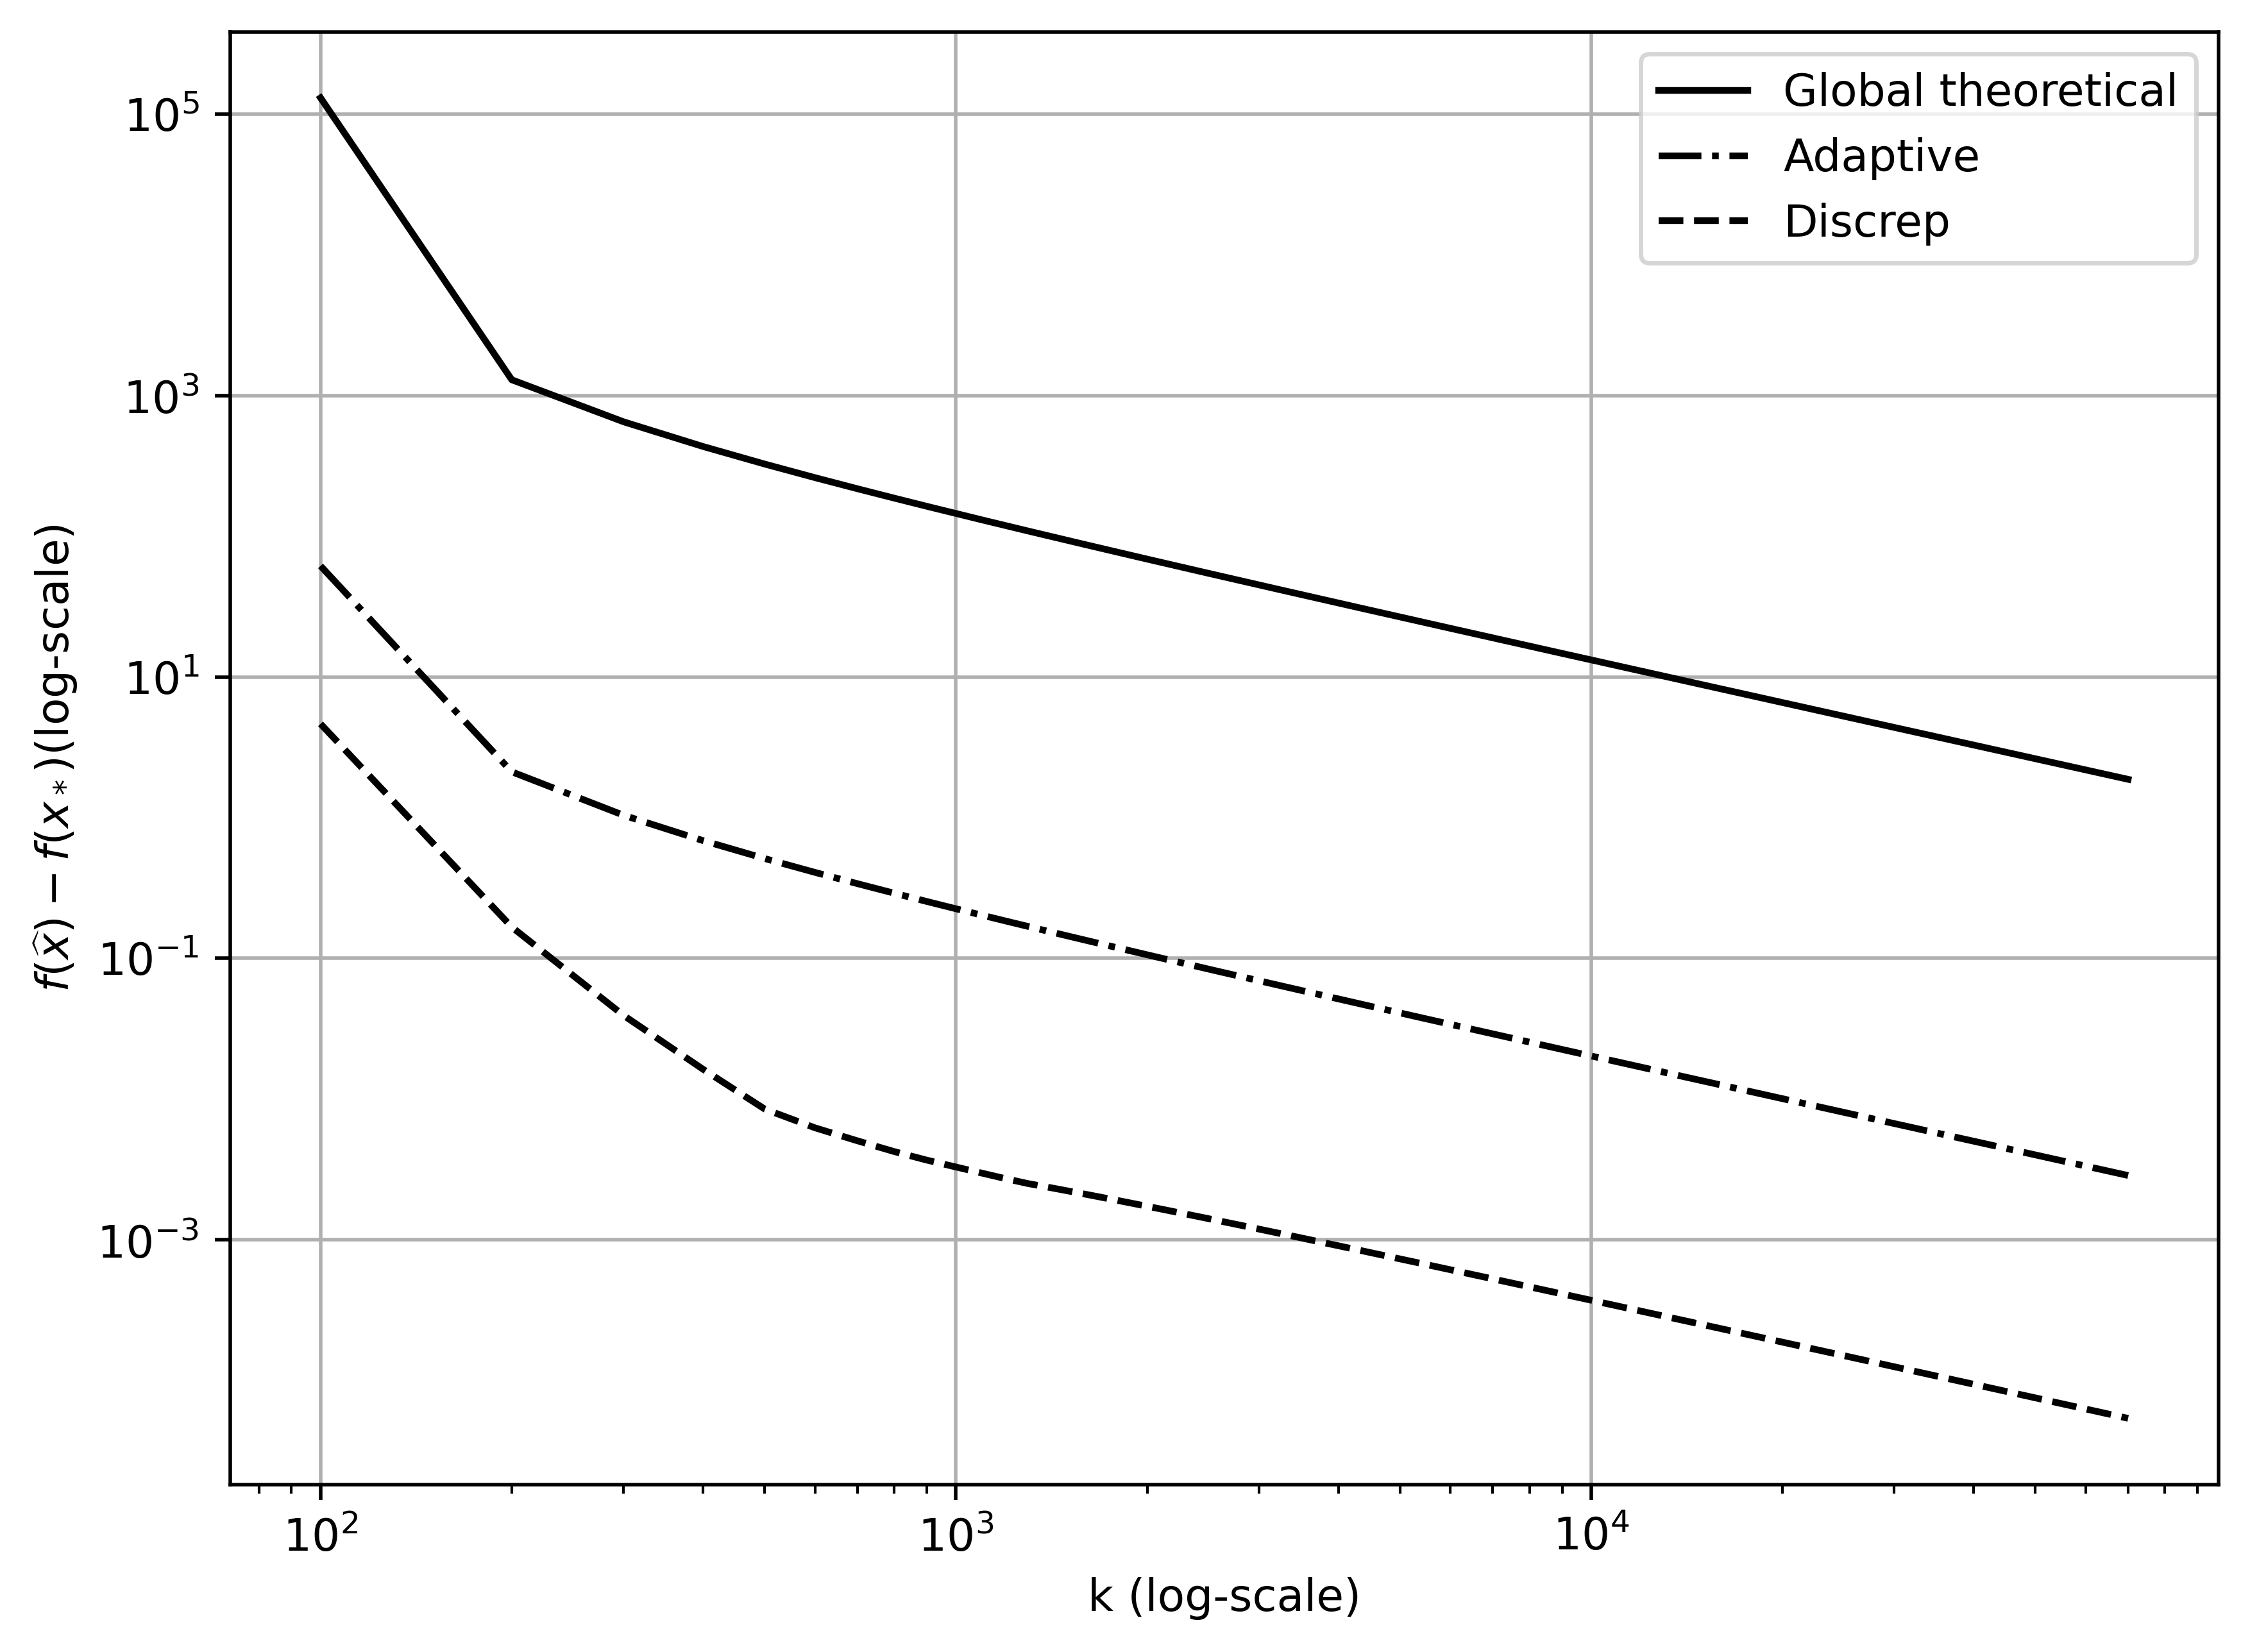
\includegraphics[width=\linewidth]{f_discr_rad_5_q_4_it_70_000_dim_1000.png}
        \endminipage\hfill
        \caption{Результаты решения задачи минимизации \eqref{sphere_cover_strongly}, учитывающей сильную выпуклость, где  $n= 1\,000, r = 5$ и  шар $Q$ радиуса 4.}
        \label{res_ex_strong_r5}
    \end{figure}

    Теперь перейдём к выпуклой постановке \eqref{sphere_cover} с целью исследования эффективности предложенного в теореме \ref{theorem1} субградиентного метода с $\Delta$-острым минимумом. К существующему набору точек, представленных для покрытия, с известным значением центра добавим дополнительную точку, которая находится вне исходного шара достаточно близко к границе (удалена не более, чем на $\Delta > 0$). Данный подход позволяет оценить <<приближённое>> значение минимума $\overline{f}$, что позволит применить указанный вариант субградиентного метода с $\Delta$-острым минимумом. При этом новое значение минимума останется внутри исходной сферы. Поскольку оптимальное значение функции --- это радиус искомого шара, покрывающего все точки, а $x_*$ всегда будет расположена внутри него, то для всякого $x$ верно неравенство $ f(x) \geq \| x - x_*\|_2$. Рассмотрим целевую функцию вида
    \begin{gather}\label{allpha_sphere_cover}
        f(x) := \alpha \max_{x\in Q}\{\|x - a_0\|_2, \|x - a_1\|_2, ..., \|x - a_m\|_2\}.
    \end{gather}
    Тогда значение $\Delta$ можно оценить  из (\ref{eq_gen_sharp}): 
        $f(x) - \overline{f} \geq \alpha\|x- x_*\|_2 - \Delta, \quad \Delta \geq \overline{f}$.

    Отметим, что данная постановка значительно влияет на величину теоретической оценки качества решения (\ref{adaptive_estimate}) для метода \eqref{orig_2}.
    Наиболее значимый вклад в оценку (\ref{adaptive_estimate}) дает последнее слагаемое $\frac{\Delta^2}{2\|\nabla f(x_k)\|^2_2}$, причём 
    $     \Delta \sim \overline{f} \sim \alpha \|\overline{x}-a\|_2 $ и 
    $     \|\nabla f(x_k)\|_2 = \alpha $. Поэтому последнее слагаемое пропорционально радиусу шара, соответствующему <<приближённому>> решению. Это и подтверждается экспериментально. Для сравнения, ниже на рис. \ref{res_sharp_convex} и \ref{res_strong_convex} приведены результаты работы для того же набора входных точек, которые необходимо покрыть в обоих постановках, (\ref{allpha_sphere_cover}) и (\ref{sphere_cover_strongly}). Начальная точка также одна и та же. Сравниваются методы из теорем \ref{theorem1} и \ref{ThmBachAdaptive}. Первый из этих методов обеспечивает сходимость буквально за 10 итераций к <<приближённому>> решению с заданной точностью и даже позволяет эту точность повысить. Второй же метод достигает схожих (с геометрической точки зрения) результатов за значительно большее количество итераций, однако он позволяет повышать точность приближённого решения на дальнейших итерациях.

    Подтверждение данного теоретического наблюдения хорошо иллюстрируется на рис. \ref{res_sharp_convex} и \ref{res_strong_convex}. На рис. \ref{res_sharp_convex} показано поведение субградиентного спуска, использующего $\Delta$-острый минимум (теорема \ref{theorem1}), а именно  быстрая сходимость к <<приближенному>> решению. Штрих-пунктирная линия соответствует оценке \eqref{eq_gen_sharp}, а штриховая --- невязке по функции и аргументу. На рис. \ref{res_strong_convex} показано поведение метода для той же задачи, но с использованием сильно выпуклого целевого функционала (теорема \ref{ThmBachAdaptive}). Скорость убывания уже не столь высокая, но точность получаемого решения в итоге выше. Сплошная линия --- это глобальная оценка \eqref{orig_estimation_f}, штрих-пунктирная --- адаптивная \eqref{adaptive_estimation_f}, а штриховая --- невязка по функции и аргументу.

    \begin{figure}[h]
        \minipage{0.49\textwidth}
        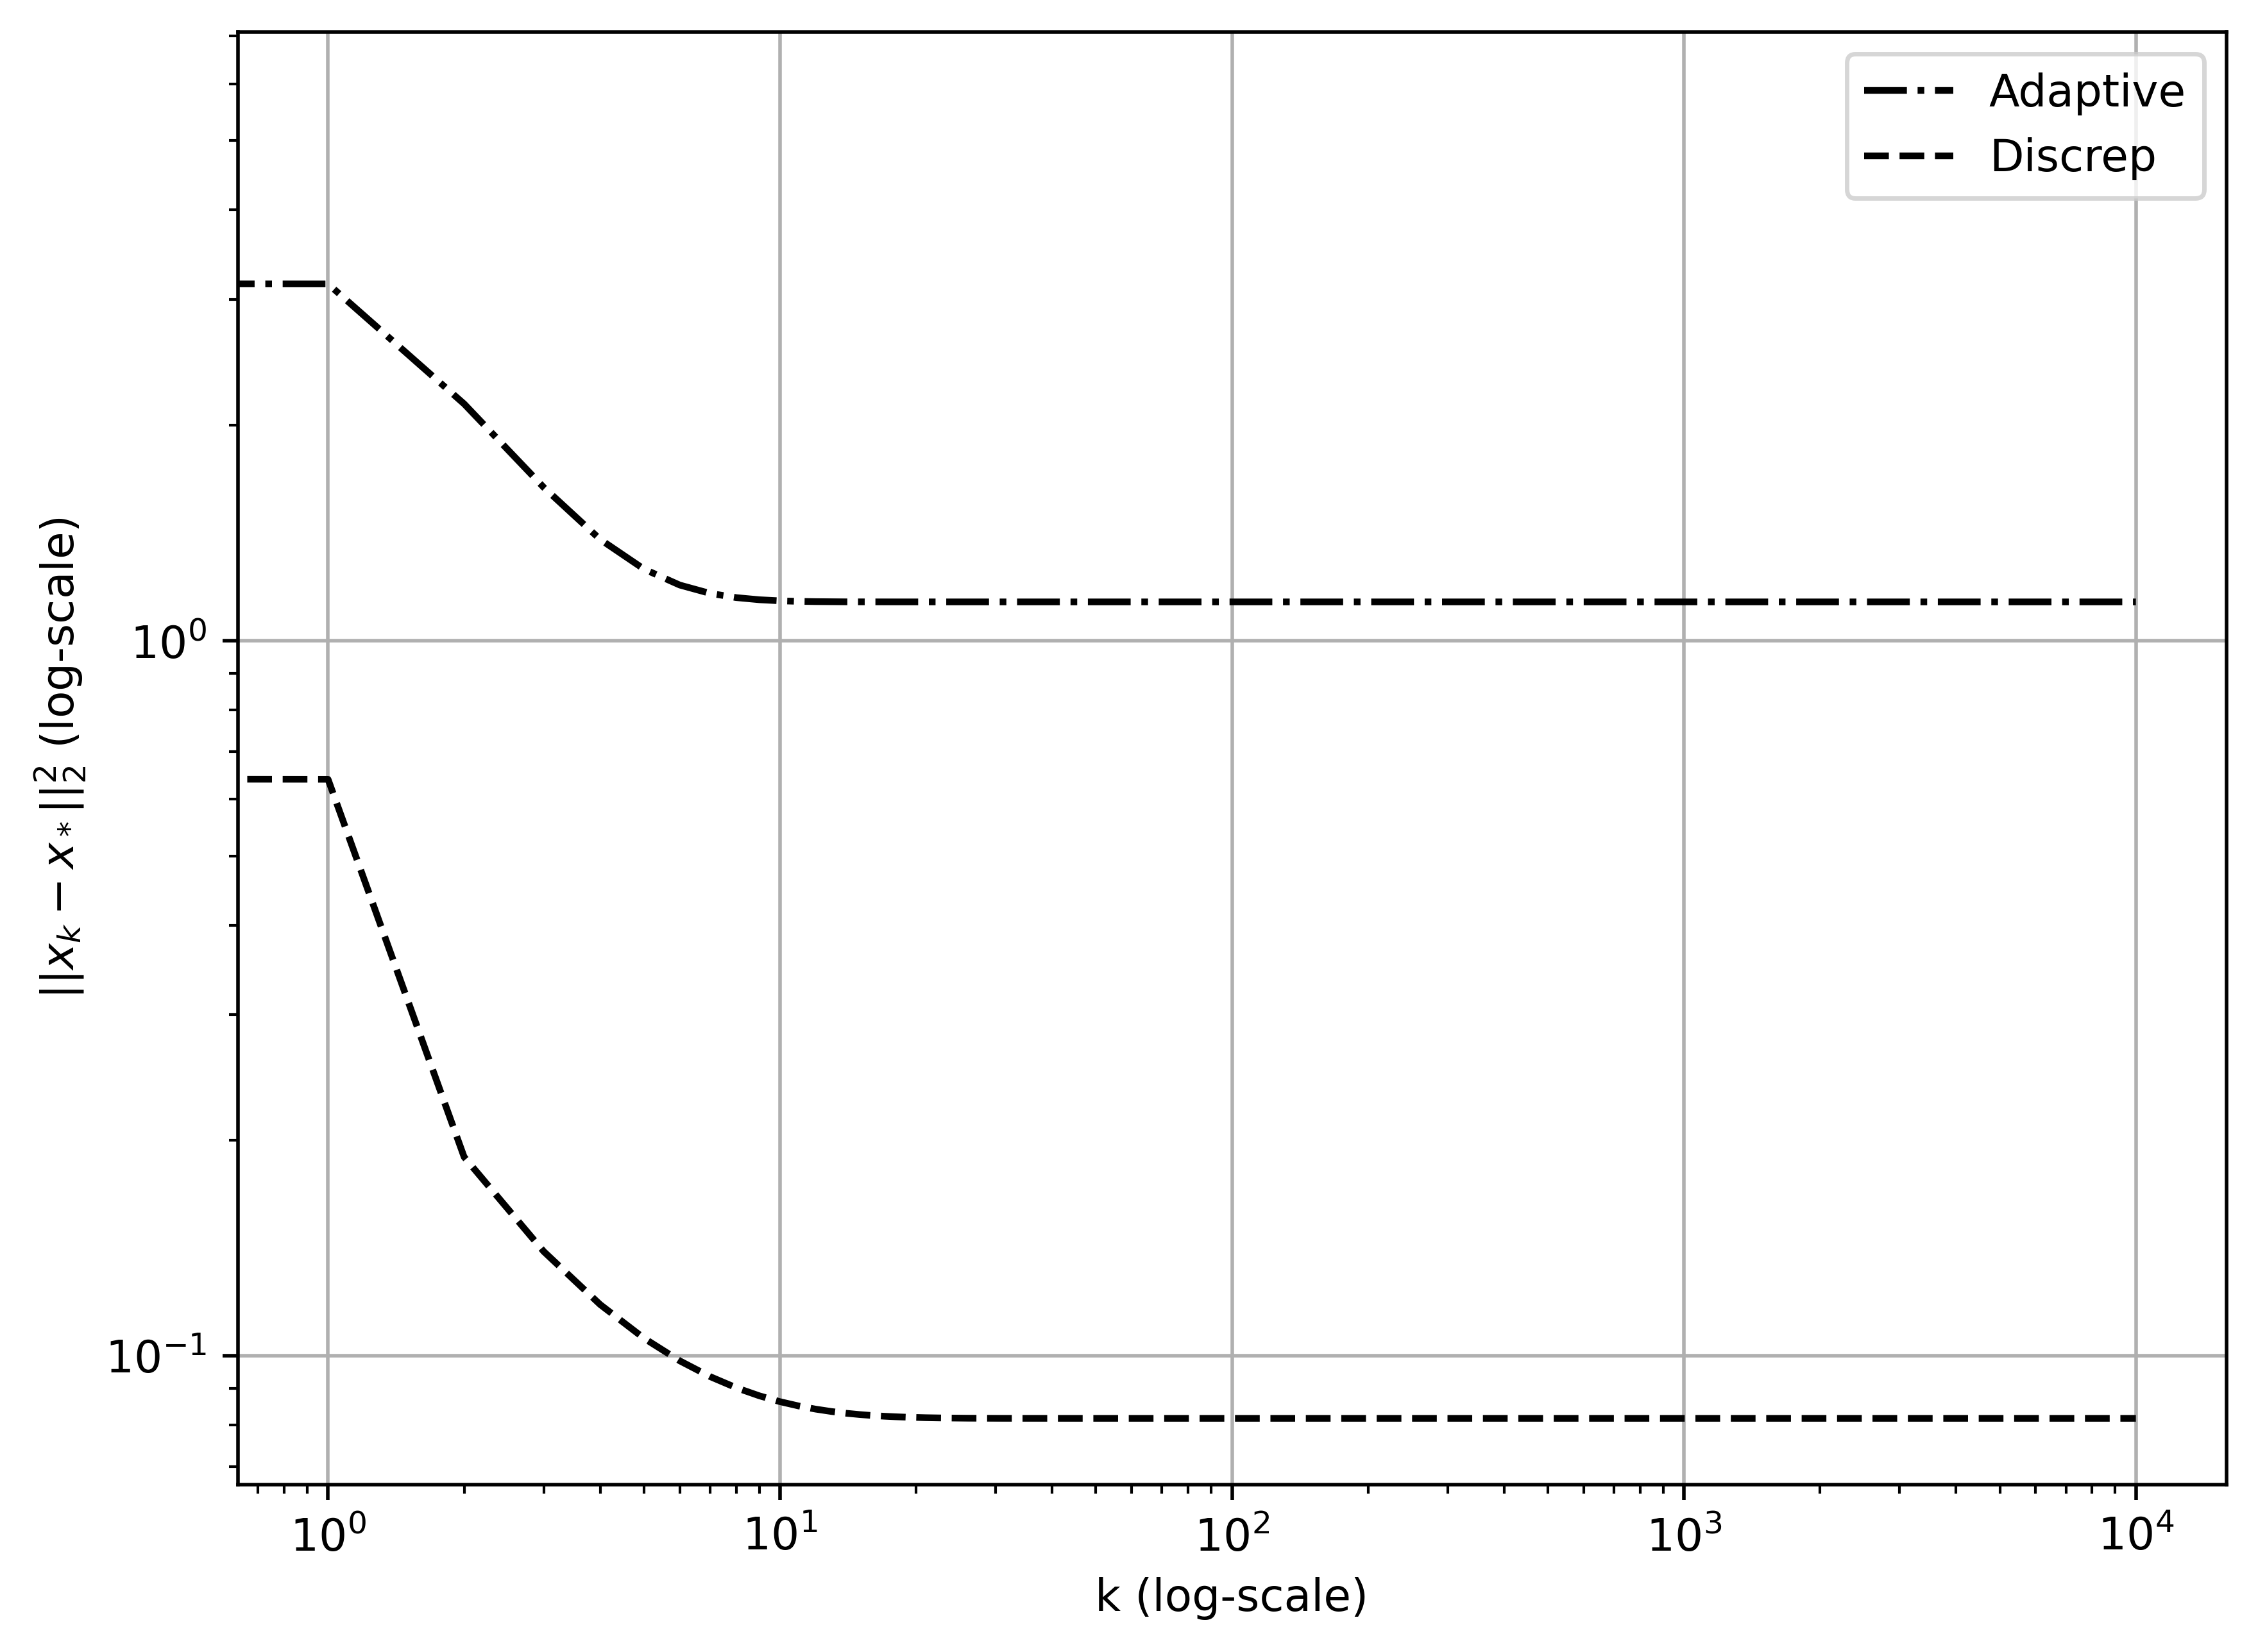
\includegraphics[width=\linewidth]{sharp_convex_x.png}
        \endminipage\hfill
        \minipage{0.49\textwidth}
        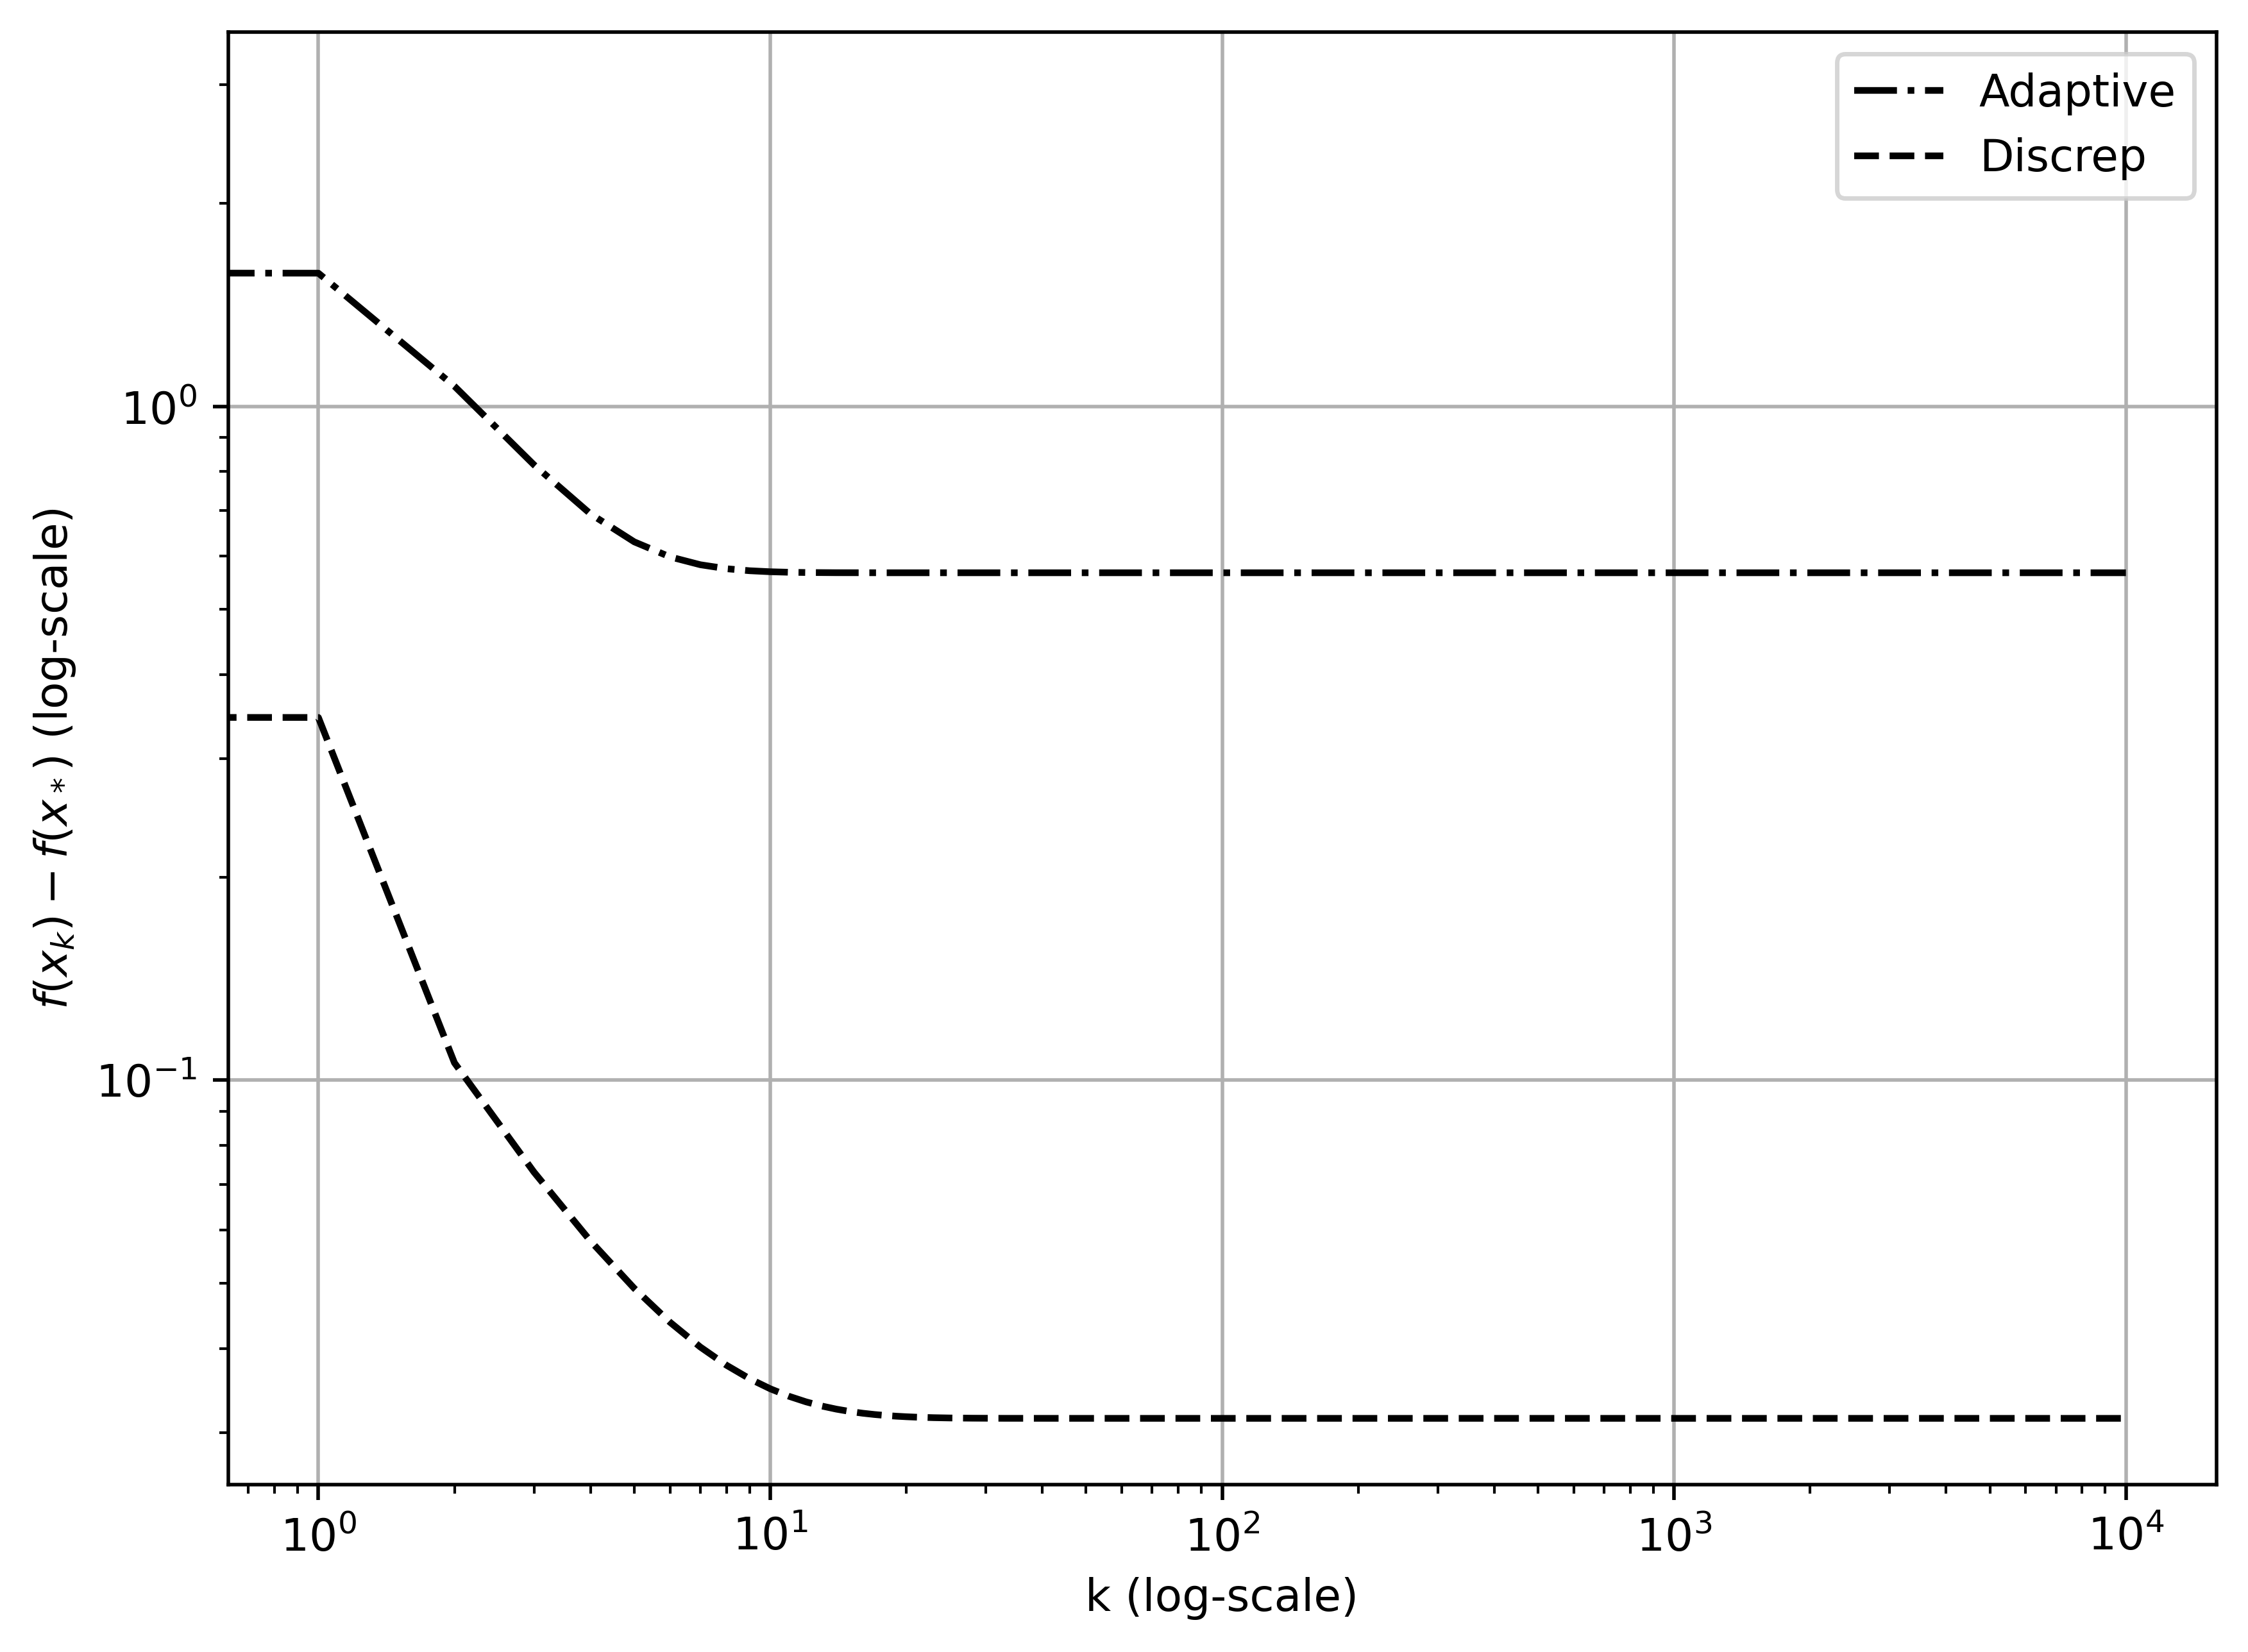
\includegraphics[width=\linewidth]{sharp_convex_f.png}
        \endminipage\hfill
        \caption{ Результаты решения задачи минимизации (\ref{allpha_sphere_cover}), учитывающей условие острого минимума, где  $n= 1\,000, r = 0.7525, \alpha = 0.6$.}
        \label{res_sharp_convex}
    \end{figure}

    \begin{figure}[h]
        \minipage{0.49\textwidth}
        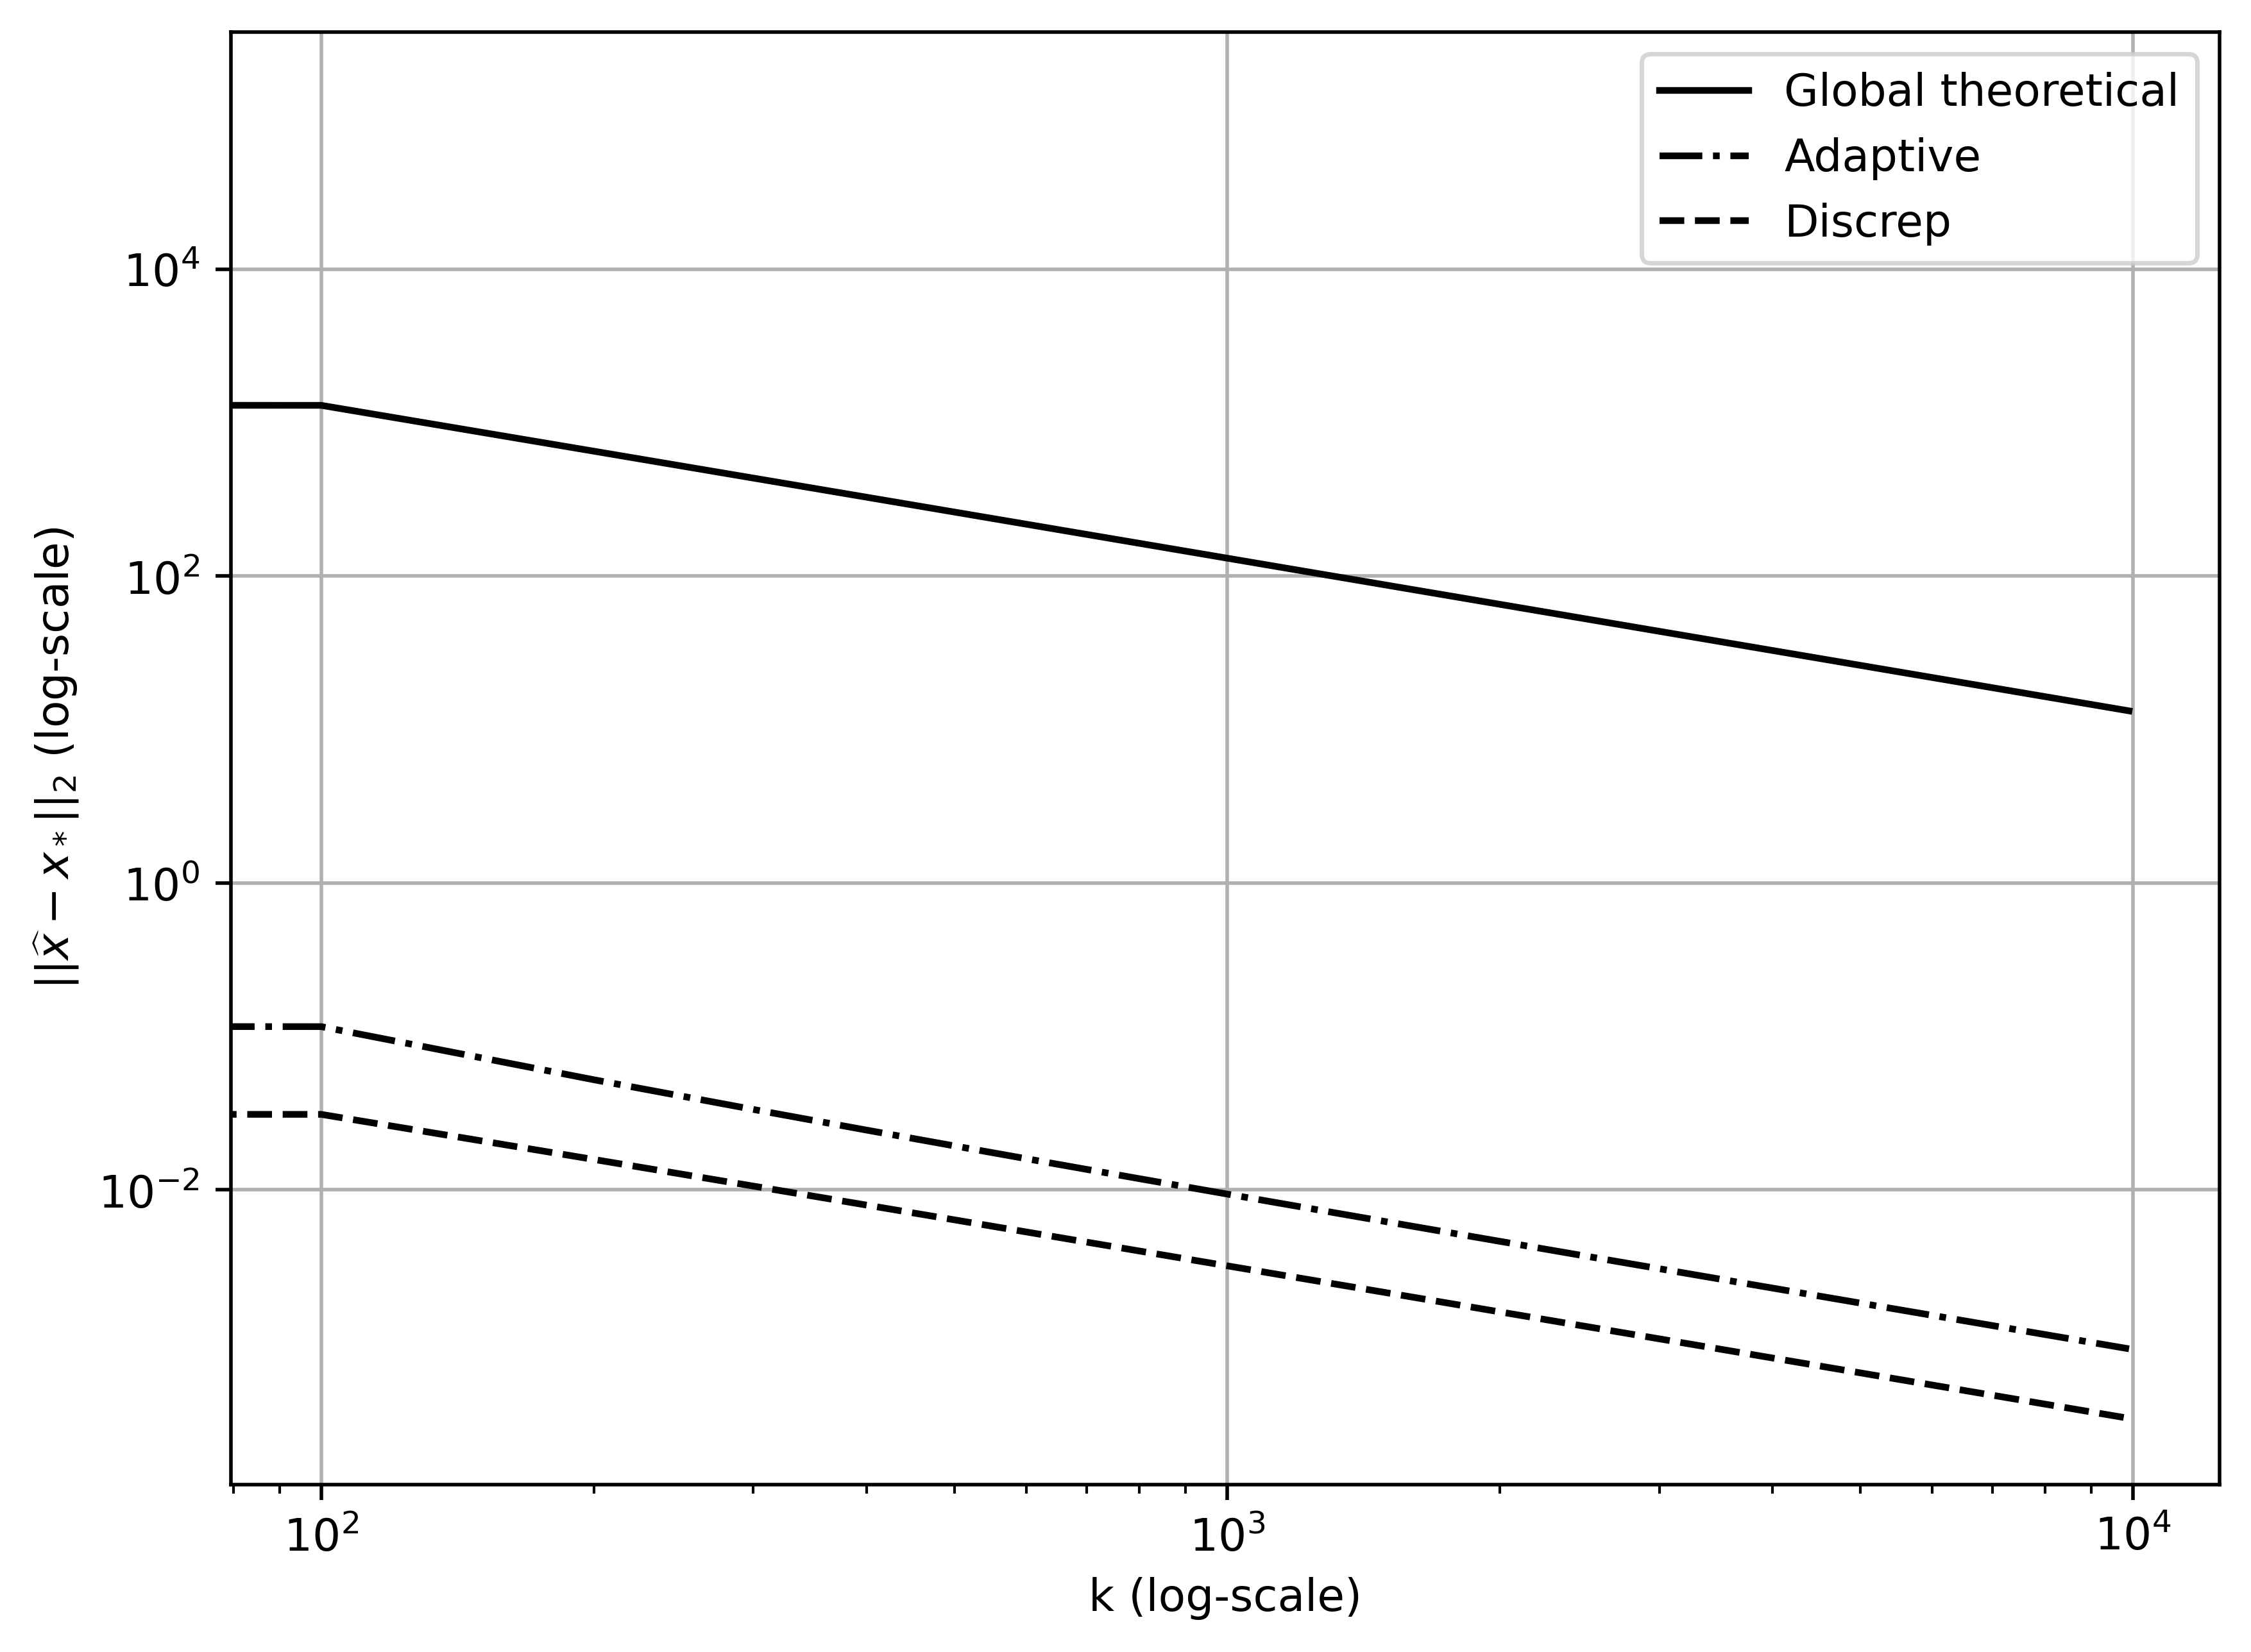
\includegraphics[width=\linewidth]{strong_convex_small_rad_x.png}
        \endminipage\hfill
        \minipage{0.49\textwidth}
        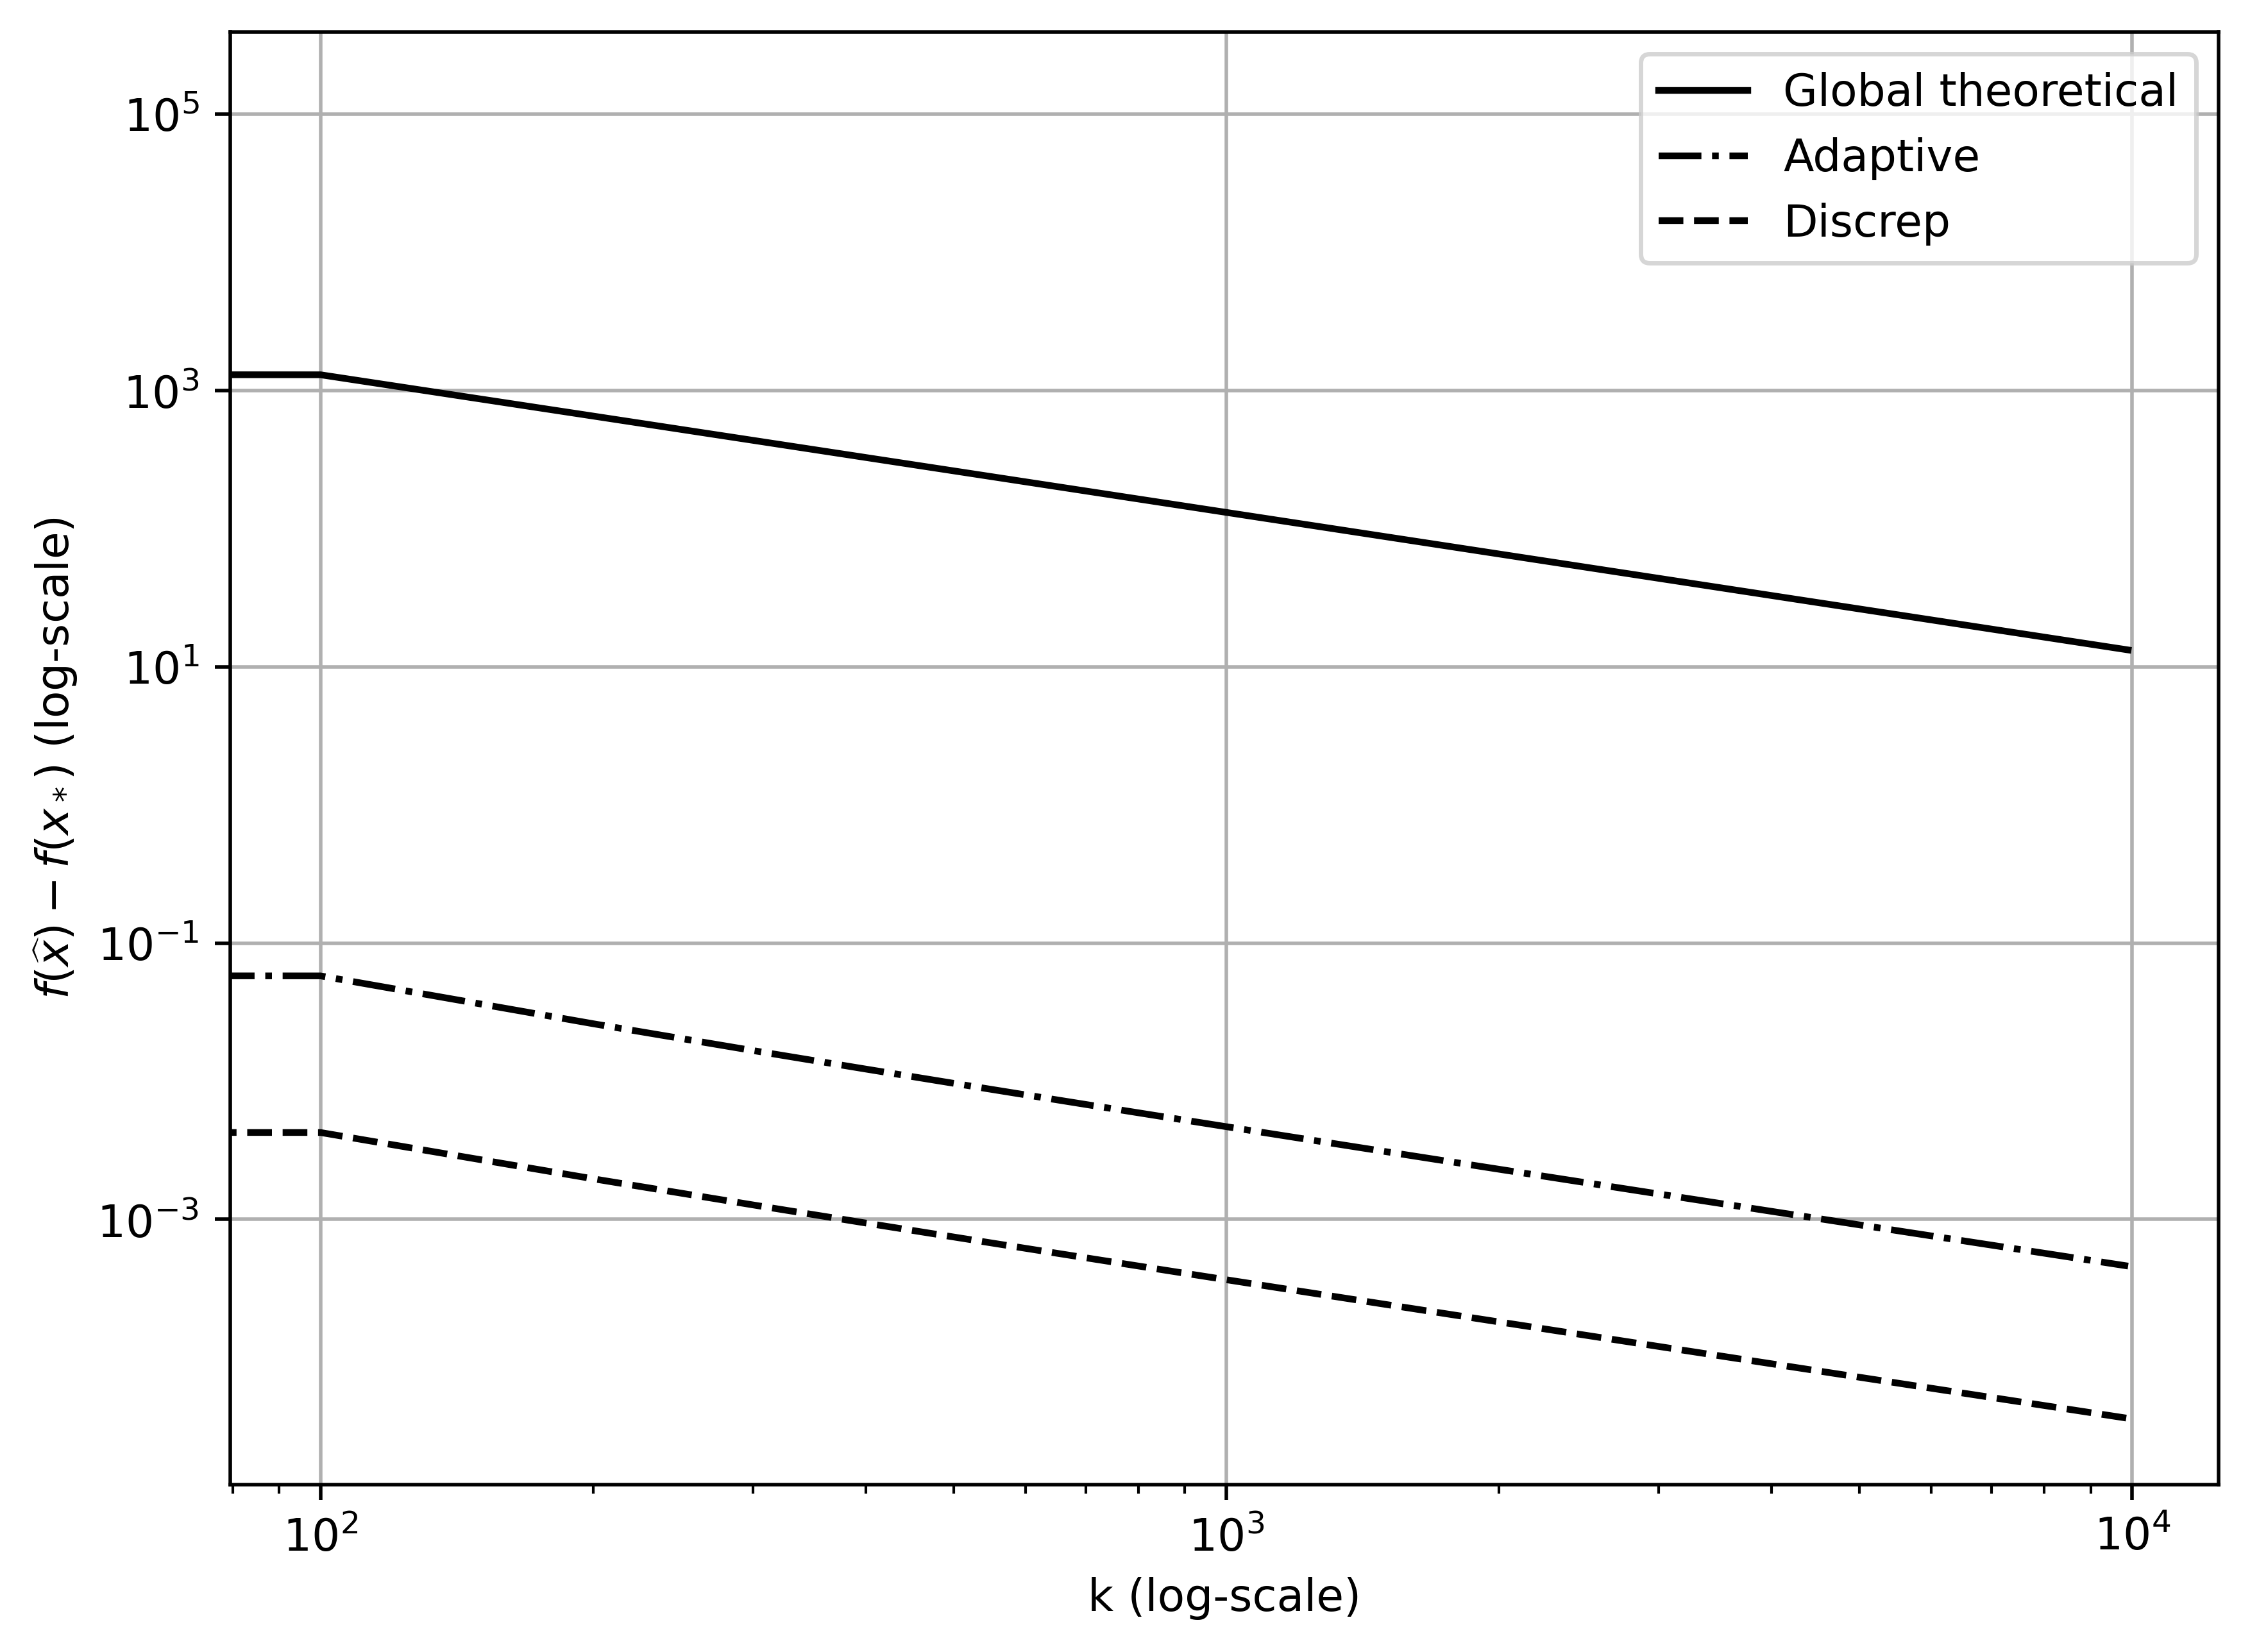
\includegraphics[width=\linewidth]{strong_convex_small_rad_f.png}
        \endminipage\hfill
        \caption{ Результаты решения задачи минимизации (\ref{sphere_cover_strongly}), учитывающей сильную выпуклость, где  $n= 1\,000, r = 0.7525$.}
        \label{res_strong_convex}
    \end{figure}

    Тем не менее, сравнение с известным точным решением $x_*$, а также график динамики значения целевой функции показывает, что за малое число шагов (значительно меньшее, чем для метода \eqref{orig_2}) реализация метода, описанного в теореме \ref{theorem1}, приводит к неплохому качеству приближённого решения. При этом, однако, для метода, учитывающего $\Delta$-острую постановку, после достижения такого уровня дальнейшее повышение качества выходной точки в отличие от метода \eqref{orig_2} уже не наблюдается. 

    Данные результаты привели к идее объединения данных подходов для достижения лучших результатов в скорости сходимости без потери возможности дальнейшего повышения точности.

\section{Рестарты зеркального спуска для выпуклых относительно липшицевых задач, удовлетворяющих условию относительного $\gamma$-роста}\label{sec:ch3/sect3}
    Техника рестартов является достаточно популярным направлением для улучшения оценок скорости сходимости при дополнительных условиях. Часто в качестве дополнительного условия выступает именно упомянутое ранее условие острого минимума (см. например \cite{sharp_rest} или часть посвященную рестартам в \cite{sharp22}).
    Воспользуемся следующим результатом (см. (6) из \cite{Lu_2018}):
    \begin{theorem} \label{vanilla_mirror}
        Пусть $f$ является выпуклой и относительно $M$-липшицевой на $Q$. Тогда можно задать метод следующим образом:
        \begin{equation} \label{mirr_upd}
            x_{k+1} = \arg \min_{x \in Q} {\left[ f(x_k) + \langle \nabla f(x_k), x - x_k \rangle + \frac{1}{h_k} V(x, x_k)\right]},
        \end{equation}
        где $\{ h_k \}$ - последовательность размеров шагов.
        Для него справедлива следующая оценка скорости сходимости:
        \begin{equation} \label{general_est}
            \min_{0\leq k \leq N} f(x_k) - f(x) \leq \frac{\frac{1}{2} M^2 \sum_{k=0}^N h_k^2 + V(x, x_0)}{\sum_{k=0}^N h_k}
        \end{equation}
    \end{theorem}
    В дальнейших рассуждениях будем обозначать 
     \[
        x_{min}^j  := \argmin_{0\leq k \leq N} f(x_k) \;\;\; \text{на} \;\; j\text{-м рестарте}.
     \]
     При $j = 0$ имеется ввиду изначальный запуск метода, использующий оригинальную стартовую точку.

    \begin{remark}
        Если в \eqref{mirr_upd} в формулировке теоремы \ref{vanilla_mirror} выбрать шаг следующим образом:
        \begin{equation} \label{mirr_step}
            h_{k} = \frac{\sqrt{2 \left[\min\limits_{x_* \in X_*}{V(x_*, x_0)}\right] }}{M\sqrt{N}},
        \end{equation}
        то можно выписать такую оценку скорости сходимости:
        \begin{equation} \label{mirr_est}
            f(x_{min}^0) - f(x_*) \leq \frac{M\sqrt{2 \left[\min\limits_{x_* \in X_*}{V(x_*, x_0)}\right]}}{\sqrt{N}}.
        \end{equation}
    \end{remark}
    Если функция обладает дополнительными свойствами, аналогичными острому минимуму,  то становится возможным применение техники рестартов. Используем аналог данного условия и вслед за Шапиро–Немировским (см. \cite{shapiro_2005} и \cite{shapiro_2021} ) введем условие относительного $\gamma$-роста ($\gamma \geq 1$). Схожее определение вводится в работе \cite{sharp_rest} (см. определение 5.2). Однако в данной работе существенно используется 1-сильная выпуклость прокс-функции. При этом в работе \cite{sharp_rest} ещё требуется условие гёльдеровости градиента или ограниченности субградиента (т.е. обычной липшицевости). Мы же в данном пункте сосредоточимся на предположении относительной липшицевости $f$. 
    
    Введём условие относительного $\gamma$-роста, позволяющее обобщить  такие условия, как острый минимум, квадратичный рост и $\gamma$-рост.
    \begin{definition}
       Будем говорить, что $f$ удовлетворяет условию относительного $\gamma$-роста, если для всякого $x \in Q$ верно неравенство:
       \begin{equation} \label{gamma-growth}
           f(x) - f(x_*) \geq \mu_{\gamma}\left(\min_{x_* \in X_*}{V(x_*,x)}\right)^{\gamma/2},
       \end{equation}
       где $X_*$ --- множество точных решений задачи минимизации $f$. 
    \end{definition}
    Существенно, что здесь не предполагается сильной выпуклости прокс-структуры. В такой общности ранее 
    рассматривался случай $\gamma = 2$ в работе \cite{gamma2}, где помимо этого предполагалась относительная гладкость целевой функции. Мы же работаем с относительно липшицевыми задачами.

    Введем следующее обозначение
    \[
        x_0^j \text{--- стартовая точка для } j\text{-го рестарта}.
    \]
    
    Справедлива следующая
    \begin{theorem} \label{simple_restart}
        Пусть $f$ удовлетворяет условию относительного $\gamma$-роста \eqref{gamma-growth} и также является относительно $M$-липшицевой на $Q$. В таком случае алгоритм \ref{alg:rest_gamma} после 
        \begin{equation}
        \begin{aligned}
           N =\mathcal{O}\left(\frac{4 M^2}{\mu_{\gamma}^2} \log_2{\left[\frac{\mu_{\gamma}^2}{\varepsilon^2} \left(\min\limits_{x_* \in X_*}{V(x_*, x_0^0)}\right) \right]}\right) \text{ при } \gamma = 1, \\
           N = \mathcal{O}\left(\frac{2^{\gamma + 1} M^2}{2^{(\gamma - 1)} - 1}\left[\frac{1}{\mu_{\gamma}^{\frac{2}{\gamma}}} \varepsilon^{\frac{2(1 - \gamma)}{\gamma}}  - \frac{1}{\mu_{\gamma}^2 \left(\min\limits_{x_* \in X_*}{V(x_*, x_0^0)}\right)^{(\gamma - 1)}} \right]\right) \text{ при } \gamma > 1,
        \end{aligned}
        \end{equation}
        обращений к субградиенту $f$ будет справедливо неравенство
        \begin{equation}
            f(x_{min}^{p-1}) - f(x_*) \leq \varepsilon.
        \end{equation}
    \end{theorem}

    \begin{algorithm}[htp]
        \caption{Рестарты зеркального спуска при условии относительного $\gamma$-роста.}
        \label{alg:rest_gamma}
        \KwData{$\varepsilon > 0$}
        \KwResult{$x_p$}
        $p \gets 0$\;
        \While{$p < \frac{1}{\gamma} \log_2{\left[\frac{\mu_{\gamma}^2}{\varepsilon^2} \left(\min\limits_{x_* \in X_*}{V(x_*, x_0^0)}\right)^{\gamma} \right]}$}{
            $x_{p}$ --- результат работы метода \eqref{mirr_upd} с шагом \eqref{mirr_step} и параметром $N_{p} = \ceil*{\frac{2^{\gamma+1} M^2}{\mu_{\gamma}^2 2^{p(1 - \gamma)}} \left(\min\limits_{x_* \in X_*}{V(x_*, x_0)}\right)^{1 - \gamma}}$\;
            $x_0 = x_{min}^p$\;
            $p=p+1$\;
        }
    \end{algorithm}

    \begin{proof}
        В доказательстве используется обозначение $x_m^n$, где $m = 0,1,...,N$ соответствует номеру итерации и $n = 0,1,...,(p-1)$ соответствует номеру рестарта метода \eqref{mirr_upd}. С учетом \eqref{gamma-growth} и \eqref{mirr_est} имеем: 
        $$
            \mu_{\gamma}\left(\min\limits_{x_* \in X_*}{V(x_*, x_{min}^0)}\right)^{\gamma/2} \leq f(x_{min}^0) - f(x_*) \leq \frac{M\sqrt{2 \min\limits_{x_* \in X_*}{V(x_*, x_0^0)}}}{\sqrt{N}}.
        $$
        Поэтому для точки выхода $x_{min}^0$ после $N_0$ итераций метода \eqref{mirr_upd}
        $$
            \mu_{\gamma}\left(\min\limits_{x_* \in X_*}{V(x_*, x_{min}^0)}\right)^{\gamma/2} \leq \frac{M\sqrt{2\min\limits_{x_* \in X_*}{V(x_*, x_0^0)}}}{\sqrt{N_0}},
        $$
        $$
            \left(\min\limits_{x_* \in X_*}{V(x_*, x_{min}^0)}\right)^{\gamma/2} \leq \frac{M\sqrt{2\min\limits_{x_* \in X_*}{V(x_*, x_0^0)}}}{\mu_{\gamma}\sqrt{N_0}},
        $$
        $$
            \min\limits_{x_* \in X_*}{V(x_*, x_{min}^0)} \leq \left(\frac{M}{\mu_{\gamma}\sqrt{N_0}}\right)^{\frac{2}{\gamma}} \left(2\min\limits_{x_* \in X_*}{V(x_*, x_0^0)}\right)^{\frac{1}{\gamma}}
        $$
        $$
            \min\limits_{x_* \in X_*}{V(x_*, x_{min}^0)} \leq \left[\min\limits_{x_* \in X_*}{V(x_*, x_0^0)} \right] \left[\frac{\sqrt{2}M}{\mu_{\gamma}\sqrt{N_0}}\right]^{\frac{2}{\gamma}} \left[\min\limits_{x_* \in X_*}{V(x_*, x_0^0)}\right]^{\frac{1}{\gamma} - 1}
        $$
        Подберем $N_0$ так, чтобы было заведомо было верно неравенство
        $$
            \left(\frac{\sqrt{2}M}{\mu_{\gamma}\sqrt{N_0}}\right)^{\frac{2}{\gamma}} \left(\min\limits_{x_* \in X_*}{V(x_*, x_0^0)}\right)^{\frac{1}{\gamma} - 1} \leq \frac{1}{2}, 
        $$
        Далее,
        $$
            \left(\frac{\sqrt{2}M}{\mu_{\gamma}}\right)^{\frac{2}{\gamma}} \left(\min\limits_{x_* \in X_*}{V(x_*, x_0^0)}\right)^{\frac{1}{\gamma} - 1} \leq \frac{1}{2} N_0^{\frac{1}{\gamma}}, 
        $$
        $$
            \frac{1}{2} N_0^{\frac{1}{\gamma}} \geq \left(\frac{\sqrt{2}M}{\mu_{\gamma}}\right)^{\frac{2}{\gamma}} \left(\min\limits_{x_* \in X_*}{V(x_*, x_0^0)}\right)^{\frac{1}{\gamma} - 1},  
        $$
        $$
            N_0 \geq 2 ^ {\gamma + 1} \frac{M^2}{\mu_{\gamma}^2} \left(\min\limits_{x_* \in X_*}{V(x_*, x_0^0)}\right)^{1 - \gamma},
        $$
        то есть
        $$
            N_0 \geq \frac{M^2 2^{\gamma + 1}}{\mu_{\gamma}^2} \left(\min\limits_{x_* \in X_*}{V(x_*, x_0^0)}\right)^{1 - \gamma}.  
        $$
        Основываясь на выписанной закономерности, проведем последовательные оценки для первых нескольких рестартов. Для 1-го рестарт метода \eqref{mirr_upd} $x_0^1 = x_{min}^0$ получаем:
        $$
            \min\limits_{x_* \in X_*}{V(x_*, x_{min}^1)} \leq \frac{1}{2} \min\limits_{x_* \in X_*}{V(x_*, x_0^1)} = \frac{1}{2} \min\limits_{x_* \in X_*}{V(x_*, x_{min}^0)} \leq \left(\frac{1}{2}\right)^2 \min\limits_{x_* \in X_*}{V(x_*, x_0^0)}
        $$
        после
        $$
            N_1 \geq \frac{M^2 2^{\gamma + 1}}{\mu_{\gamma}^2} \left(\min\limits_{x_* \in X_*}{V(x_*, x_0^1)}\right)^{1 - \gamma} \geq \frac{M^2 2^{\gamma + 1}}{\mu_{\gamma}^2} \left(\min\limits_{x_* \in X_*}{V(x_*, x_{min}^0)}\right)^{1 - \gamma} 
        $$
        обращений к алгоритму \eqref{mirr_upd} при $\gamma > 1$. Поэтому
        $$
            \min\limits_{x_* \in X_*}{V(x_*, x_{min}^0)} \leq \frac{1}{2}\min\limits_{x_* \in X_*}{V(x_*, x_0^0)},
        $$
        $$
            \left(\min\limits_{x_* \in X_*}{V(x_*, x_{min}^0)}\right)^{\gamma - 1} \leq \left(\frac{1}{2} \min\limits_{x_* \in X_*}{V(x_*, x_0^0)}\right)^{\gamma - 1},
        $$
        $$
             \left(\frac{1}{2} \min\limits_{x_* \in X_*}{V(x_*, x_0^0)}\right)^{1 - \gamma} \leq \left(\min\limits_{x_* \in X_*}{V(x_*, x_{min}^0)}\right)^{1 - \gamma}.
        $$
        Это означает, что
        $$
        \begin{aligned}
            N_1 \geq \frac{M^2 2^{\gamma + 1}}{\mu_{\gamma}^2} \left(\min\limits_{x_* \in X_*}{V(x_*, x_{min}^0)}\right)^{1 - \gamma} \geq \frac{M^2 2^{\gamma + 1}}{\mu_{\gamma}^2} \left(\frac{1}{2} \min\limits_{x_* \in X_*}{V(x_*, x_0^0)}\right)^{1 - \gamma} =\\
            = \frac{M^2 2^{\gamma + 1}}{\mu_{\gamma}^2 2^{1-\gamma}} \left(\min\limits_{x_* \in X_*}{V(x_*, x_0^0)}\right)^{1 - \gamma}.
        \end{aligned}
        $$
        Далее, для 2-го рестарта имеем $x_0^2 = x_{min}^1$. Тогда
        $$
            \min\limits_{x_* \in X_*}{V(x_*, x_{min}^2)} \leq \frac{1}{2} \min\limits_{x_* \in X_*}{V(x_*, x_0^2)} \leq \left(\frac{1}{2}\right)^3 \min\limits_{x_* \in X_*}{V(x_*, x_0^0)} 
        $$
        после не более, чем $N_2$ обращений к субградиенту целевой функции $f$, где
        $$
        \begin{aligned}
            N_2 \geq \frac{M^2 2^{\gamma + 1}}{\mu_{\gamma}^2} \left(\min\limits_{x_* \in X_*}{V(x_*, x_0^2)}\right)^{1 - \gamma} = \frac{M^2 2^{\gamma + 1}}{\mu_{\gamma}^2} \left(\min\limits_{x_* \in X_*}{V(x_*, x_{min}^1)}\right)^{1 - \gamma} \geq\\
            \geq \frac{M^2 2^{\gamma + 1}}{\mu_{\gamma}^2 2^{1 - \gamma}} \left(\min\limits_{x_* \in X_*}{V(x_*, x_0^1)}\right)^{1 - \gamma} \geq \frac{M^2 2^{\gamma + 1}}{\mu_{\gamma}^2 2^{2(1 - \gamma)}} \left(\min\limits_{x_* \in X_*}{V(x_*, x_0^0)}\right)^{1 - \gamma}.
        \end{aligned}
        $$
        Наконец, для $(p-1)$-го рестарта имеем:
        \begin{equation} \label{v_seq}
            \min\limits_{x_* \in X_*}{V(x_*, x_{min}^{p - 1})} \leq \frac{1}{2^p} \min\limits_{x_* \in X_*}{V(x_*, x_0^0)}
        \end{equation}
        после
        \begin{equation} \label{n_seq}
            N_{p-1} \geq \frac{M^2 2^{\gamma + 1}}{\mu_{\gamma}^2 2^{(p - 1)(1 - \gamma)}} \left(\min\limits_{x_* \in X_*}{V(x_*, x_0^0)}\right)^{1 - \gamma}.
        \end{equation}
        Используя найденную зависимость \eqref{n_seq}, оценим общее число обращений к оракулу (здесь предполагается, что $\gamma > 1$, случай $\gamma = 1$ рассмотрим далее):
        \begin{equation} \label{n_p_sum}
        \begin{aligned}
            \sum_{k=0}^{p - 1} N_k \geq \frac{M^2 2^{\gamma + 1}}{\mu_{\gamma}^2} \left(\min\limits_{x_* \in X_*}{V(x_*, x_0^0)}\right)^{1 - \gamma} (1 + 2^{(\gamma-1)} + 2^{2(\gamma - 1)} + ... + 2^{(p-1)(\gamma - 1)}) = \\
            = \frac{M^2 2^{\gamma + 1}}{\mu_{\gamma}^2} \frac{1 - 2^{p(\gamma-1)}}{1 - 2^{(\gamma-1)}} \left(\min\limits_{x_* \in X_*}{V(x_*, x_0^0)}\right)^{1 - \gamma}.
        \end{aligned}
        \end{equation}
        Теперь оценим невязку по функции:
        $$
            f(x_{min}^{p-1}) - f(x_*) \leq \frac{M\sqrt{2\min\limits_{x_* \in X_*}{V(x_*, x_{p-1}^0)}}}{\sqrt{N_{p-1}}} \leq \sqrt{\frac{M^2 \frac{2}{2^{p-1}} \min\limits_{x_* \in X_*}{V(x_*, x_0^0)}}{N_{p-1}}} \leq
        $$
        $$
            \leq \sqrt{\frac{M^2 \frac{1}{2^{p-2}} \min\limits_{x_* \in X_*}{V(x_*, x_0^0)}}{\frac{M^2 2^{\gamma + 1}}{\mu_{\gamma}^2 2^{(p - 1)(1 - \gamma)}} \left(\min\limits_{x_* \in X_*}{V(x_*, x_0^0)}\right)^{1 - \gamma}}} = \sqrt{\frac{ \mu_{\gamma}^2 2^{(p - 1)(1 - \gamma)} }{2^{p-2} 2^{\gamma + 1} \left(\min\limits_{x_* \in X_*}{V(x_*, x_0^0)}\right)^{- \gamma}}} = 
        $$
        $$
            = \sqrt{\mu_{\gamma}^2 2^{p - 1 - p\gamma + \gamma - p + 2 - \gamma - 1} \left(\min\limits_{x_* \in X_*}{V(x_*, x_0^0)}\right)^{\gamma}} = \sqrt{\frac{\mu_{\gamma}^2} {2^{p\gamma}} \left(\min\limits_{x_* \in X_*}{V(x_*, x_0^0)}\right)^{\gamma}}.
        $$
        Необходимо добиться того, чтобы $f(x_{min}^{p-1}) - f(x_*) \leq \varepsilon$. Для этого достаточно потребовать
        $$
            \frac{\mu_{\gamma}^2}{\varepsilon^2} \left(\min\limits_{x_* \in X_*}{V(x_*, x_0^0)}\right)^{\gamma} \leq 2^{p\gamma},
        $$
        откуда и получаем необходимую оценку количества рестартов метода \eqref{mirr_upd}:
        \begin{equation} \label{p_rest}
            p \geq \frac{1}{\gamma} \log_2{\left[\frac{\mu_{\gamma}^2}{\varepsilon^2} \left(\min\limits_{x_* \in X_*}{V(x_*, x_0^0)}\right)^{\gamma} \right]}.
        \end{equation}
        Сопоставив \eqref{p_rest} и \eqref{n_p_sum}, выпишем общую оценку количества обращений к оракулу:
        $$
            \sum_{k=0}^{p-1} N_k \geq \frac{M^2 2^{\gamma + 1}}{\mu_{\gamma}^2} \cdot \frac{2^{p(\gamma-1)} - 1}{2^{(\gamma-1)} - 1} \left(\min\limits_{x_* \in X_*}{V(x_*, x_0^0)}\right)^{1 - \gamma} \geq 
        $$
        $$
            \geq \frac{M^2 2^{\gamma + 1}}{\mu_{\gamma}^2 (2^{(\gamma-1)} - 1)} \left(\left[\frac{\mu_{\gamma}^2}{\varepsilon^2} \left(\min\limits_{x_* \in X_*}{V(x_*, x_0^0)}\right)^{\gamma}\right]^{\frac{\gamma - 1}{\gamma}} - 1\right) \left(\min\limits_{x_* \in X_*}{V(x_*, x_0^0)}\right)^{1 - \gamma} =
        $$
        $$
            = \frac{2^{\gamma + 1} M^2}{\mu_{\gamma}^2 (2^{(\gamma - 1)} - 1)}\left(\left[\frac{\mu_{\gamma}^2}{\varepsilon^2}\right]^{\frac{\gamma - 1}{\gamma}} - \frac{1}{\left(\min\limits_{x_* \in X_*}{V(x_*, x_0^0)}\right)^{(\gamma - 1)}} \right) =
        $$
        $$
            = \frac{2^{\gamma + 1} M^2}{\mu_{\gamma}^2 (2^{(\gamma - 1)} - 1)}\left(\left[\frac{\mu_{\gamma}^2}{\varepsilon^2}\right]^{\frac{\gamma - 1}{\gamma}} - \frac{1}{\left(\min\limits_{x_* \in X_*}{V(x_*, x_0^0)}\right)^{(\gamma - 1)}} \right) =
        $$
        $$
            = \frac{2^{\gamma+1} M^2}{2^{(\gamma - 1)} - 1}\left(\frac{1}{\mu_{\gamma}^{\frac{2}{\gamma}}} \varepsilon^{\frac{2(1 - \gamma)}{\gamma}}  - \frac{1}{\mu_{\gamma}^2 \left(\min\limits_{x_* \in X_*}{V(x_*, x_0^0)}\right)^{(\gamma - 1)}} \right).
        $$
        Отдельно рассмотрим случай, когда $\gamma = 1$:
        $$
        \begin{aligned}
            \sum_{k=0}^{p-1} N_k = \ceil*{\frac{4 p M^2}{\mu_{\gamma}^2}} \geq \frac{4 M^2}{\gamma\mu_{\gamma}^2} \log_2{\left[\frac{\mu_{\gamma}^2}{\varepsilon^2} \left(\min\limits_{x_* \in X_*}{V(x_*, x_0^0)}\right)^{\gamma} \right]} = \\
            = \frac{4 M^2}{\mu_{\gamma}^2} \log_2{\left[\frac{\mu_{\gamma}^2}{\varepsilon^2} \left(\min\limits_{x_* \in X_*}{V(x_*, x_0^0)}\right) \right]}
        \end{aligned}
        $$
        Таким образом, получаем следующие оценки для количества итераций, необходимых для достижения желаемой точности:
        $$
            \mathcal{O} \left(\frac{4 M^2}{\mu_{\gamma}^2} \log_2{\left[\frac{\mu_{\gamma}^2}{\varepsilon^2} \left(\min\limits_{x_* \in X_*}{V(x_*, x_0^0)}\right) \right]}\right) \text{ при } \gamma = 1,
        $$
        $$
            \mathcal{O} \left(\frac{2^{\gamma + 1} M^2}{2^{(\gamma - 1)} - 1}\left[\frac{1}{\mu_{\gamma}^{\frac{2}{\gamma}}} \varepsilon^{\frac{2(1 - \gamma)}{\gamma}}  - \frac{1}{\mu_{\gamma}^2 \left(\min\limits_{x_* \in X_*}{V(x_*, x_0^0)}\right)^{(\gamma - 1)}} \right]\right) \text{ при } \gamma > 1.
        $$
    \end{proof}

\section{Адаптивный критерий остановки каждого из рестартов зеркального спуска для липшицевых задач с относительным $\gamma$-ростом}\label{sec:ch3/sect4}

    Оказывается, что при некоторых дополнительных предположениях возможно построить адаптивный вариант зеркального спуска в предыдущем пункте. Воспользуемся результатом, полученным в замечании \ref{remark4} к лемме \ref{th:base}. При помощи данного результата проведем замену глобальной константы $M$ на локальные значения в теореме \ref{vanilla_mirror}. Начнем со вспомогательного утверждения (см. теорему 5.3.1 из \cite{nemirovskyLectures})
    \begin{proposition} \label{adapt_mirror}
        Пусть $f$ является выпуклой и $M$-липшицевой на $Q$, причем прокс-функция $d(x)$ является 1-сильно выпуклой.
        Зададим метод аналогично теореме \ref{vanilla_mirror}: 
        \begin{equation} \label{adapt_upd}
            x_{k+1} = \arg \min_{x \in Q} {\left[ f(x_k) + \langle \nabla f(x_k), x - x_k \rangle + \frac{1}{h_k} V(x, x_k)\right]},
        \end{equation}
        где $\{ h_k \}$ последовательность размеров шагов. Тогда справедлива следующая оценка:
        \begin{equation} \label{adapt_est}
            \min_{0\leq k \leq N} f(x_k) - f(x_*) \leq \frac{\sum_{k=0}^N h_k^2 \norm{\nabla f(x_k)}^2_*} {2 \sum_{k=0}^N h_k} + \frac{\min\limits_{x_* \in X_*}{V(x_*, x_0)} }{\sum_{k=0}^N h_k}.
        \end{equation}
    \end{proposition}

    На практике для использования приведенной выше теоремы \ref{simple_restart} требуется знать величину $\min\limits_{x_* \in X_*}{V(x_*, x_0)}$, что делает проблемным применимость метода на практике. Потому введем $\Theta$ следующим образом
    $$
        \Theta^2 \geq \min\limits_{x_* \in X_*}{V(x_*, x_0)}.
    $$
    Тогда \eqref{adapt_est} означает, что 
    \begin{equation} \label{adapt_est_theta}
    \begin{aligned}
        \min_{0\leq k \leq N} f(x_k) - f(x_*) \leq \frac{\sum_{k=0}^N h_k^2 \norm{\nabla f(x_k)}^2_*} {2 \sum_{k=0}^N h_k} + \frac{\min\limits_{x_* \in X_*}{V(x_*, x_0)} }{\sum_{k=0}^N h_k} \leq \\
        \leq \frac{\sum_{k=0}^N h_k^2 \norm{\nabla f(x_k)}^2_*} {2 \sum_{k=0}^N h_k} + \frac{\Theta^2}{\sum_{k=0}^N h_k}.
    \end{aligned}
    \end{equation}
    Отметим, что класс липшицевых задач с аналогом условия относительно $\gamma$-роста рассматривался ранее, например в \cite{sharp_rest}, однако предлагаемое ниже в алгоритме \ref{alg:rest_criteria} адаптивное правило рестарта предложено впервые. Отметим следующее наблюдение (см. например \cite{Bayandina2018}).
    \begin{remark}
        Если в \eqref{adapt_upd} выбрать шаг следующим образом:
        \begin{equation} \label{eps_step}
            h_{k} = \frac{\varepsilon}{\norm{\nabla f(x_k)}^2_*},
        \end{equation}
        и воспользоваться критерием остановки метода: 
        \begin{equation} \label{stop_crit}
            \sum_{k=0}^N \frac{1} {\norm{\nabla f(x_k)}^2_*} \geq \frac{2 \Theta^2}{\varepsilon^2}, \;\;\;\;\text{ где } \Theta^2 \geq \min\limits_{x_* \in X_*}{V(x_*, x_0)},
        \end{equation}
        тогда для невязки по функции можно показать следующее (прямое следствие \eqref{adapt_est_theta}):
        \begin{equation} 
        \begin{aligned}
            \min_{0\leq k \leq N} f(x_k) - f(x_*) \leq \frac{\varepsilon}{2} + \frac{\Theta^2}{\varepsilon \sum_{k=0}^N \frac{1} {\norm{\nabla f(x_k)}^2_*}} \leq \varepsilon.
        \end{aligned}
        \end{equation}
     \end{remark}
     Предложим следующий алгоритм \ref{alg:rest_criteria}. 
     \begin{algorithm}[htp]
        \caption{Рестарты зеркального спуска при условии $\gamma$-роста с критерием остановки.}
        \label{alg:rest_criteria}
        \KwData{$\varepsilon > 0$}
        \KwResult{$x_p$}
        $p \gets 0$\;
        $\Theta_0^2 \geq \min\limits_{x_* \in X_*}{V(x_*,x_0)}$\;
        \While{$p < \log_2{\left[\left(\frac{\mu_{\gamma}}{\varepsilon}\right)^{\frac{2}{\gamma}} \Theta_0^2\right]}$}{
            $x_{p}$ --- результат работы метода \eqref{mirr_upd} с шагом \eqref{eps_step} и критерием остановки $\sum_{k=0}^{N_p} \frac{1}{\norm{\nabla f(x_k) }_*^2} \geq \frac{ 2^{(p \gamma - p  + 1)}}{\mu_{\gamma}^2 \Theta_0^{2\gamma - 2} }$, где $N_p$ --- количество итераций на данном рестарте метода\;
            $x_0 = x_{min}^p$\;
            $p=p+1$\;
        }
    \end{algorithm}
    \begin{theorem}
        Пусть $f$ выпукла и удовлетворяет условию относительного $\gamma$-роста \eqref{gamma-growth} с 1-сильно выпуклой прокс-структурой, а также является $M$-липшицевой на $Q$. В таком случае после работы алгоритма \ref{alg:rest_criteria} будет справедливо неравенство
        \begin{equation}
            f(x_{min}^{p-1}) - f(x_*) \leq \varepsilon.
        \end{equation}
        Для этого потребуется не более чем
        \begin{equation}
           N = \mathcal{O} \left( \frac{4 M^2}{\mu_{\gamma}^2} \log_2{\left[\frac{\mu_{\gamma}^2 \Theta_0^2}{\varepsilon^2} \right]} \right) \text{ при } \gamma = 1
        \end{equation}
        или
        \begin{equation}
           N = \mathcal{O}\left( \frac{2^{(\gamma + 1)} M^2 }{2^{(\gamma - 1)} - 1}\left[ \frac{1}{\mu_{\gamma}^{\frac{2}{\gamma}}} \varepsilon^{\frac{2}{\gamma} - 2} - \frac{1}{\mu_{\gamma}^2 \Theta_0^{2(\gamma - 1)}} \right] \right) \text{ при } \gamma > 1
        \end{equation}
        обращений к оракулу, где $\Theta_0^2$ --- это оценка сверху для $\min\limits_{x_* \in X_*}{V(x_*, x_0)}$.
    \end{theorem}

    \begin{proof}
       Воспользуемся предположением:
       $$
           \min\limits_{x_* \in X_*}{V(x_*, x_0)} \leq \Theta_0^2
       $$
       Выберем $\varepsilon_0$ так, чтобы 
       $$
       \begin{aligned}
           \mu_{\gamma}\left(\min\limits_{x_* \in X_*}{V(x_*, x_{min}^0)}\right)^{\gamma/2} \leq f(x_{min}^0) - f(x_*) \leq \mu_{\gamma}\left(\frac{\min\limits_{x_* \in X_*}{V(x_*, x_{min}^0)}}{2}\right)^{\gamma/2} \leq \\
           \leq \varepsilon_0 := \mu_{\gamma}\left(\frac{\Theta_0^2}{2}\right)^{\gamma/2} = \frac{\mu_{\gamma}}{\sqrt{2^{\gamma}}}\Theta_0^{\gamma},
       \end{aligned}
       $$
       \[
           \text{ т.е.   } \varepsilon_0 = \frac{\mu_{\gamma}}{\sqrt{2^{\gamma}}}\Theta_0^{\gamma}.
       \]
       Тогда
       $$
           \mu_{\gamma}\left(\min\limits_{x_* \in X_*}{V(x_*, x_{min}^0)}\right)^{\gamma/2} \leq \frac{\mu_{\gamma}}{\sqrt{2^{\gamma}}}\Theta_0^{\gamma},
       $$
       $$
           \left(\min\limits_{x_* \in X_*}{V(x_*, x_{min}^0)}\right)^{\gamma} \leq \frac{\Theta_0^{2\gamma}}{2^{\gamma}},
       $$
       $$
           \left(\min\limits_{x_* \in X_*}{V(x_*, x_{min}^0)}\right)^{\gamma} \leq \left(\frac{\Theta_0^2}{2}\right)^{\gamma}.
       $$
       Ввиду $\gamma \geq 1$ получаем
       $$
           \min\limits_{x_* \in X_*}{V(x_*, x_{min}^0)} \leq \frac{\Theta_0^2}{2}.
       $$
       С учетом критерия остановки алгоритма \eqref{adapt_upd} на $0$-м рестарте получаем
       \begin{equation} \label{krit}
           \sum_{k=0}^{N_0} \frac{1}{\norm{\nabla f(x_k) }_*^2} \geq \frac{2 \Theta_0^2}{\varepsilon_0^2} = \frac{2 \Theta_0^2}{{\frac{\mu_{\gamma}^2 \Theta_0^{2\gamma}}{2^{\gamma}}}} = \frac{2^{\gamma + 1}}{\mu_{\gamma}^2 \Theta_0^{2\gamma - 2}}.
       \end{equation}
       Если $\norm{\nabla f(x_k) }_* \leq M$, то
       \[
           \sum_{k=0}^{N_0} \frac{1}{\norm{\nabla f(x_k) }_*^2} \geq \frac{N_0}{M^2}.
       \]
       Значит критерий остановки \eqref{krit} будет заведомо выполнен при
       \[
            \sum_{k=0}^{N_0} \frac{1}{\norm{\nabla f(x_k) }_*^2} \geq \frac{N_0}{M^2} \geq \frac{2^{\gamma + 1}}{\mu_{\gamma}^2 \Theta_0^{2\gamma - 2}},
       \]
       откуда
       $$
            N_0 \geq \frac{2^{\gamma + 1} M^2}{\mu_{\gamma}^2 \Theta_0^{2\gamma - 2}}.
       $$
       Для последующих рестартов введем вспомогательные оценки $\Theta_i$:
       \[
           \Theta_1 = \frac{\Theta_0}{\sqrt{2}}
       \]
       \[
           \Theta_2 = \frac{\Theta_1}{\sqrt{2}} = \frac{\Theta_0}{(\sqrt{2})^2}
       \]
       \[
           ...
       \]
       \[
           \Theta_p = \frac{\Theta_0}{(\sqrt{2})^p}
       \]
       Поэтому для второго рестарта справедливо следующее:
       \[
           \min\limits_{x_* \in X_*}{V(x_*, x_{0}^1)} \leq \Theta_1^2,
       \]
       \[
           \min\limits_{x_* \in X_*}{V(x_*, x_{0}^2)} = \min\limits_{x_* \in X_*}{V(x_*, x_{min}^1)} \leq \frac{\Theta_1^2}{2},
       \]
       а для третьего перезапуска, соответственно:
       \[
           \min\limits_{x_* \in X_*}{V(x_*, x_{0}^2)} \leq \Theta_2^2.
       \]
       Проведем те же рассуждения в общем виде для $(p-1)$-го рестарта:
       \[
           \varepsilon_{p-1} := \mu_{\gamma} \left(\frac{\Theta_{p-1}^2}{2}\right)^{\frac{\gamma}{2}} = \mu_{\gamma} \left(\frac{\Theta_0^2}{2^{p}}\right)^{\frac{\gamma}{2}},
       \]
       и тогда имеем: 
       \[
           \mu_{\gamma}\left(\min\limits_{x_* \in X_*}{V(x_*, x_{min}^{p-1})}\right)^{\frac{\gamma}{2}} \leq f(x_{min}^{p-1}) - f(x_*) \leq \varepsilon_{p-1},
       \]
       откуда
       \[
           \min\limits_{x_* \in X_*}{V(x_*, x_{min}^{p-1})} \leq \frac{\Theta_0^2}{2^p}.
       \]
       Вспомним соответствующий критерий остановки алгоритма \eqref{adapt_upd} на $(p-1)$-м рестарте:
       \[
           \sum_{k=0}^{N_{p-1}} \frac{1}{\norm{\nabla f(x_k) }_*^2} \geq \frac{2 \Theta_{p-1}^2}{\varepsilon_{p-1}^2} = \frac{2 \Theta_0^2}{{2^{p-1} \mu_{\gamma}^2 \frac{ \Theta_0^{2\gamma}}{2^{p\gamma}}}} = \frac{1}{\mu_{\gamma}^2 \Theta_0^{2\gamma - 2} 2^{(p - \gamma p - 1)}}.
       \]
       Он заведомо выполнен при
       \[
           \sum_{k=0}^{N_{p-1}} \frac{1}{\norm{\nabla f(x_k) }_*^2} \geq \frac{N_{p-1}}{M^2} \geq \frac{1}{\mu_{\gamma}^2 \Theta_0^{2\gamma - 2} 2^{(p - \gamma p - 1)}},
       \]
       т.е. при 
       \[
           N_{p-1} \geq \frac{M^2}{\mu_{\gamma}^2 \Theta_0^{2\gamma - 2} 2^{(p - \gamma p - 1)}} = \frac{2 M^2}{\mu_{\gamma}^2 \Theta_0^{2\gamma - 2} } 2^{p(\gamma - 1)}.
       \]
       \iffalse
       Используя полученное неравенство мы получаем следующую оценку для $N_p$:
       \[
            N_p \geq \frac{2 \cdot 2^{\gamma} \cdot 2^{p\gamma} M^2}{2^p \mu_{\gamma}^2} \min\limits_{x_* \in X_*}{V(x_*, x_0)}^{(1 - \gamma)}
       \]
       \fi
       Используя данный подход получим следующую оценку (достаточно завышенную):
       \[
        \begin{aligned}
           \sum_{k=0}^{p-1} N_k \geq \frac{M^2 2^{(\gamma + 1)}}{\mu_{\gamma}^2 \Theta_0^{2(\gamma - 1)} } (1 + 2^{(\gamma-1)} + 2^{2(\gamma - 1)} + ... + 2^{(p-1)(\gamma - 1)}) = \\
           = \frac{M^2 2^{(\gamma + 1)}}{\mu_{\gamma}^2 \Theta_0^{2(\gamma - 1)}} \frac{1 - 2^{p(\gamma-1)}}{1 - 2^{(\gamma-1)}}.
       \end{aligned}
       \]
       При $\gamma = 1$ имеем:
       \[
           \sum_{k=0}^{p-1} N_k = \ceil*{\frac{4 p M^2}{\mu_{\gamma}^2}}.
       \]
       Для финальной оценки необходимо получить оценку для количества рестартов $(p-1)$, обозначим $\varepsilon \geq \varepsilon_{p-1}$, то есть финальную, необходимую точность:
       \[
           \varepsilon \geq \varepsilon_{p-1} = \mu_{\gamma} \left(\frac{\Theta_0^2}{2^{p}}\right)^{\frac{\gamma}{2}},
       \]
       \[
           \left(\frac{\varepsilon}{\mu_{\gamma}}\right)^{\frac{2}{\gamma}} \geq  \frac{\Theta_0^2}{2^p},
       \]
       \[
            2^p \geq \left(\frac{\mu_{\gamma}}{\varepsilon}\right)^{\frac{2}{\gamma}} \Theta_0^2,
       \]
       \[
            p \geq \log_2{\left[\left(\frac{\mu_{\gamma}}{\varepsilon}\right)^{\frac{2}{\gamma}} \Theta_0^2\right]}.
       \]
       Соответственно, при $\gamma > 1$:
       \[
       \begin{aligned}
           \sum_{k=0}^{p-1} N_k \geq & \frac{M^2 2^{(\gamma + 1)}}{\mu_{\gamma}^2 \Theta_0^{2(\gamma - 1)}} \frac{2^{p(\gamma-1)} - 1}{2^{(\gamma-1)} - 1} \geq \\
           \geq& \frac{M^2 2^{(\gamma + 1)}}{\mu_{\gamma}^2 \Theta_0^{2(\gamma - 1)} (2^{(\gamma-1)} - 1)} \left[\left(\left[\frac{\mu_{\gamma}}{\varepsilon}\right]^{\frac{2}{\gamma}} \Theta_0^2\right) ^{(\gamma-1)} - 1\right] = \\
           =& \frac{M^2 2^{(\gamma + 1)}}{\mu_{\gamma}^2 (2^{(\gamma-1)} - 1) \Theta_0^{2(\gamma - 1)}} \left(\frac{\mu_{\gamma}}{\varepsilon}\right)^{\frac{2\gamma - 2}{\gamma}} \Theta_0^{2\gamma - 2} - \frac{M^2 2^{(\gamma + 1)}}{\mu_{\gamma}^2 (2^{(\gamma-1)} - 1) \Theta_0^{2(\gamma - 1)}} = \\ 
           =& \frac{2^{(\gamma + 1)} M^2 }{\cancel{\mu_{\gamma}^2} (2^{(\gamma-1)} - 1) \cancel{\Theta_0^{2(\gamma - 1)}}} \cdot\frac{\cancel{\mu_{\gamma}^2} \cdot \mu_{\gamma}^{- \frac{2}{\gamma}} }{\varepsilon^{2- \frac{2}{\gamma}}} \cancel{\Theta_0^{2\gamma - 2}} - \frac{2^{(\gamma + 1)} M^2 }{\mu_{\gamma}^2 (2^{(\gamma - 1)} - 1) \Theta_0^{2(\gamma - 1)}} = \\
           =& \frac{2^{(\gamma + 1)} M^2 }{2^{(\gamma - 1)} - 1}\left( \frac{1}{\mu_{\gamma}^{\frac{2}{\gamma}}} \varepsilon^{\frac{2}{\gamma} - 2} - \frac{1}{\mu_{\gamma}^2 \Theta_0^{2(\gamma - 1)}} \right) 
       \end{aligned}
       \]
       И при $\gamma = 1$:
       \[
           \sum_{k=0}^{p-1} N_k = \ceil*{\frac{4 p M^2}{\mu_{\gamma}^2}} \geq \frac{4 M^2}{\mu_{\gamma}^2} \log_2{\left[\left(\frac{\mu_{\gamma}}{\varepsilon}\right)^{\frac{2}{\gamma}} \Theta_0^2\right]} = \frac{4 M^2}{\mu_{\gamma}^2} \log_2{\left[\frac{\mu_{\gamma}^2 \Theta_0^2}{\varepsilon^2} \right]} 
       \]
       Таким образом, получаем следующие оценки общего количества обращений к оракулу:
       \[
           \mathcal{O} \left( \frac{4 M^2}{\mu_{\gamma}^2} \log_2{\left[\frac{\mu_{\gamma}^2 \Theta_0^2}{\varepsilon^2} \right]} \right) \text{ при } \gamma = 1,
       \]
       \[
           \mathcal{O} \left( \frac{2^{(\gamma + 1)} M^2 }{2^{(\gamma - 1)} - 1}\left[ \frac{1}{\mu_{\gamma}^{\frac{2}{\gamma}}} \varepsilon^{\frac{2}{\gamma} - 2} - \frac{1}{\mu_{\gamma}^2 \Theta_0^{2(\gamma - 1)}} \right] \right) \text{ при } \gamma > 1 .
       \]
       
       \iffalse
           Соответственно при $\gamma > 1$, степень $1 - \gamma$ является отрицательной, потому справедливо следующее изменение оценки \eqref{eq:v_sup}:
           \begin{equation}
               V(x_*, x_{min}^p)^{(1 - \gamma)} \geq (\frac{V(x_*, x_0^p)}{2})^{(1 - \gamma)} \geq \frac{V(x_*, x_0^0)^{(1 - \gamma)}}{2^{p(1 - \gamma)} 2^{(1 - \gamma)}}
           \end{equation}
           то есть: 
           \begin{equation}
               V(x_*, x_0^p)^{(1 - \gamma)} \geq \frac{V(x_*, x_0^0)^{(1 - \gamma)} 2^{(1-\gamma)}}{2^{p(1 - \gamma)} 2^{(1 - \gamma)}} = \frac{V(x_*, x_0^0)^{(1 - \gamma)}}{2^{p(1 - \gamma)}}
           \end{equation}
           Используя полученное неравенство мы получаем следующую оценку для $N_p$:
           \begin{equation}
                N_p \geq \frac{2^{\gamma + 1} M^2}{\mu_{\gamma}^2} V(x_*, x_0^p)^{(1 - \gamma)} \geq  \frac{2^{\gamma + 1} M^2}{\mu_{\gamma}^2} \frac{V(x_*, x_0^0)^{(1 - \gamma)}}{2^{p(1 - \gamma)}} = \frac{2 \cdot 2^{\gamma} \cdot 2^{p\gamma} M^2}{2^p \mu_{\gamma}^2} V(x_*, x_0^0)^{(1 - \gamma)}
           \end{equation}
           Используя данный подход получим следующую оценку (достаточно завышенную):
           $$
               \sum_{k=1}^{p} N_k \geq \frac{2 \cdot 2^{\gamma} M^2}{\mu_{\gamma}^2} V(x_*, x_0^0)^{(1 - \gamma)} (1 + 2^{(\gamma-1)} + 2^{2(\gamma - 1)} + ... + 2^{p(\gamma - 1)}) = \frac{2 \cdot 2^{\gamma} M^2}{\mu_{\gamma}^2} \frac{1 - 2^{p(\gamma-1)}}{1 - 2^{(\gamma-1)}} (V(x_*, x_0^0))^{1 - \gamma}
           $$
           Так же отдельно рассмотрим случай $\gamma = 1$:
           $$
               \sum_{k=1}^{p} N_k = \frac{4 p M^2}{\mu_{\gamma}^2} 
           $$
           Для финальной оценки необходимо получить оценку для количества рестартов $p$, обозначим $\varepsilon := \varepsilon_p$ - то есть финальную, необходимую точность:
           \begin{equation}
               \varepsilon = \varepsilon_p = \mu_{\gamma} (\frac{V(x_*, x_0^p)}{2})^{\frac{\gamma}{2}} \leq  \mu_{\gamma} (\frac{V(x_*, x_0^0)}{2^{p+1}})^{\frac{\gamma}{2}}
           \end{equation}
           \begin{equation}
               (\frac{\varepsilon}{\mu_{\gamma}})^{\frac{2}{\gamma}} \leq  \frac{V(x_*, x_0^0)}{2 \cdot 2^p}
           \end{equation}
           \begin{equation}
               (\frac{\varepsilon}{\mu_{\gamma}})^{\frac{2}{\gamma}} \leq  \frac{V(x_*, x_0^0)}{2 \cdot 2^p}
           \end{equation}
           Критерий?:
           \begin{equation}
               V(x_*, x_0^p) \leq \frac{1}{2} \sum_{k=0}^N \frac{\varepsilon_p^2}{\norm{\nabla f(x_k) }_2^2} \leq \frac{\varepsilon_p^2}{2} \frac{N_p}{M^2}
           \end{equation}
       \fi
    \end{proof}

    Полученный результат имеет схожие оценки с предыдущей теоремой \ref{simple_restart}, однако на практике критерий остановки может значительно сократить количество итераций, необходимых для достижения заданной точности $\varepsilon$. Также при помощи данного метода легко прогнозируется точность перед каждым рестартом метода, что удобно для контроля за правильностью работы метода. Также подобная информация позволяет переключаться между несколькими модификациями метода, изменяющими, например, параметр $\Theta_0$. Оптимизация данного параметра позволит улучшить оценки без модификации самого метода, что позволит встроить его в более комплексные адаптивные фреймворки в дальнейшем. 
\FloatBarrier